\documentclass[fleqn,10pt]{wlscirep}

\usepackage[utf8]{inputenc}
\usepackage[T1]{fontenc}
\usepackage{times}
\usepackage{epsfig}
\usepackage{graphicx}
\usepackage{amsmath}
\usepackage{amssymb}
\usepackage{soul}
\usepackage{xcolor}
\usepackage{mathbbol}
\usepackage{multicol}
\usepackage[numbers,sort&compress]{natbib}

\newcommand{\NCMRGBR}{29,051\,}
\newcommand{\NCALLS}{801,526\,} % Number of genotyped SNPs 
\newcommand{\MAFTHR}{1\% } % MAF threshold (in percentage)
\newcommand{\NIMP}{9472708} % number of % number of imputed variants with MAF > threshold
\newcommand{\HWEPVAL}{$10^{-5}$} % Hardy-Weinberg equilibrium p-value threshold
\newcommand{\LVNP}{2,677} % number of points in the LV mesh
\newcommand{\NGWASHITS}{10}

% ANONYMISED VERSION 
% \newcommand{\ACCESSIONNUMBER}{---}

\newcommand{\ACCESSIONNUMBER}{11350}

\title{Unsupervised deep learning helps disentangle the genetic basis of cardiac morphology}

\author[1,2,*]{Rodrigo Bonazzola}
\author[1,2]{Nishant Ravikumar}
\author[1,2]{Avan Suinesiaputra}
\author[6,7]{Bernard Keavney}
\author[2]{Sven Plein}
\author[3]{Enzo Ferrante}
\author[4]{Tanveer Syeda-Mahmood}
\author[1,2,5]{Alejandro F Frangi}
\affil[1]{Centre for Computational Imaging and Simulation Technologies in Biomedicine (CISTIB), School of Computing and School of Medicine, University of Leeds, Leeds, UK}
\affil[2]{Leeds Institute of Cardiovascular and Metabolic Medicine, School of Medicine, University of Leeds, Leeds, UK}
\affil[3]{Research Institute for Signals, Systems and Computational Intelligence, sinc(i), FICH-UNL / CONICET, Santa Fe, Argentina}
\affil[4]{IBM Almaden Research Center, San Jose, USA}
\affil[5]{Medical Imaging Research Center (MIRC), University Hospital Gasthuisberg. Cardiovascular Sciences and Electrical Engineering Departments, KU Leuven, Leuven, Belgium}
\affil[6]{Division of Cardiovascular Sciences, Faculty of Biology, Medicine and Health, University of Manchester, Manchester, UK}
\affil[7]{Manchester University NHS Foundation Trust, Manchester Academic Health Science Centre, Manchester, UK}

\affil[*]{scrb@leeds.ac.uk}


\begin{abstract}
Recent studies have identified associations between genetic variants and simple cardiac parameters like the volume of heart chambers or myocardial thickness. The emergence of big databases, including genetic data linked to cardiac magnetic resonance (CMR) images, with high spatial and temporal resolution facilitates investigation of more nuanced shape patterns.. However, the high dimensionality of these images makes it challenging to find associations with genetic variants of potential clinical relevance. In this work, we exploit the UK Biobank database to extract left-ventricular geometric features from image-derived 3D meshes in an unsupervised fashion, via convolutional mesh autoencoders. These features are then tested in a genome-wide association study in order to unravel the genetic basis of cardiac morphology. Our results shed light on the role of gene phospholamban (PLN) in cardiac shape variation. In particular, our approach allowed to find a link between this gene and LV sphericity which had not been reported previously.

% Recent studies have identified associations between genetic variants and simple cardiac parameters like the volume of heart chambers or myocardial thickness. The emergence of big databases, including genetic data linked to cardiac magnetic resonance (CMR) images, with high spatial and temporal resolution provides the means to describe more complex shape patterns. However, the high dimensionality of these images makes it challenging to find associations with genetic variants of potential clinical relevance. In this work, we propose a framework which combines geometric deep learning with genome-wide association studies to disclose novel links between cardiac anatomy and the underlying genetic basis. We construct convolutional mesh autoencoders to learn low-dimensional representations of cardiac meshes, and show that such embeddings encode anatomical variations linked to genetic differences. Our experimental results demonstrate that the proposed framework not only finds well-known genetic associations for cardiac shape changes, but also reveals novel links which open the door for future biomedical research.
\end{abstract}

\begin{document}

\flushbottom
\maketitle

\thispagestyle{empty}

% % \noindent Please note: Abbreviations should be introduced at the first mention in the main text – no abbreviations lists. Suggested structure of main text (not enforced) is provided below.

% \noindent\textbf{Color legend (for revisers):}\newline
\textcolor{red}{- Comments to coauthors who will revise this manuscript.}\newline
\textcolor{gray}{- Reminders of work yet to be done.}\newline
\textcolor{green}{- Statements for which evidence is yet needed.}\newline
\textcolor{blue}{- Statements that need to be supported by specific literature}\newline
\textcolor{purple}{- This color means I am still trying to find a better way to say the same}\newline

\nopagebreak


\section*{Introduction}
Genome-wide association studies (GWAS) have remarkably accelerated discoveries of associations between genomic and complex traits ~\cite{ref_gwas_review}. These studies analyse genetic variants (i.e the genotype) in a sample of individuals, to test if any of these variants are associated with the presence of disease or with systematic changes in measurable traits, known broadly as phenotypes. GWAS have been extremely successful in identifying genetic variants associated with a broad range of diseases and other complex traits, such as metabolic, anthropometric or behavioral ones. These findings have improved our understanding of the pathogenesis of a disease, allowing us to develop better treatments, supporting drug discovery, and advance towards precision medicine.

With large-scale epidemiological imaging studies, GWAS have been applied to image-derived phenotypes (IDP), linking genetic with physiological processes of internal organs. In cardiology, the most common IDPs to associate with genetic variants are features like volumes, mass and function indices derived from the left ventricle (LV)~\cite{ref_nayaung, ref_biffi}, as the diagnosis of patients with heart disease typically starts from quantitative analysis of this cardiac chamber. Although there are discrepancies on the number of genetic loci associated with changes in LV IDPs from recently reported GWAS \cite{ref_nayaung, ref_pirruccello, ref_biffi}, some consistent genetic factors have been established. 
For instance, \cite{ref_nayaung} and \cite{ref_pirruccello} have both identified that TTN ({\em titin}) gene is strongly associated with LV end-diastolic and end-systolic volumes, which consequently associated also with ejection fraction. TTN is responsible for the sarcomere assembly of the myocytes, which determines stretching, contraction and passive stiffness of the myocardium~\cite{granzier_giant_2004}. Protein-truncating TTN variants have also been shown to be responsible for dilated cardiomyopathy (DCM) ~\cite{tayal_phenotype_2017}.

These cardiac imaging genetics studies are based on a traditional approach, where handcrafted features characterising LV IDPs were first determined before running GWAS to find the associated genetic loci. Although these IDPs have been clinically used to diagnose heart disease, they do not provide a detailed representation of tissue morphology and its variation across the population. In this paper, we advance the view that shape features encoded in a learned latent space can be a powerful way to correlate with genetic information in GWAS studies. The fact that they reveal more detailed cardiac indices than traditional volume measurements is also supported by atlas-based studies~\cite{gilbert_independent_2019, medrano-gracia_left_2014}.

\begin{figure*}
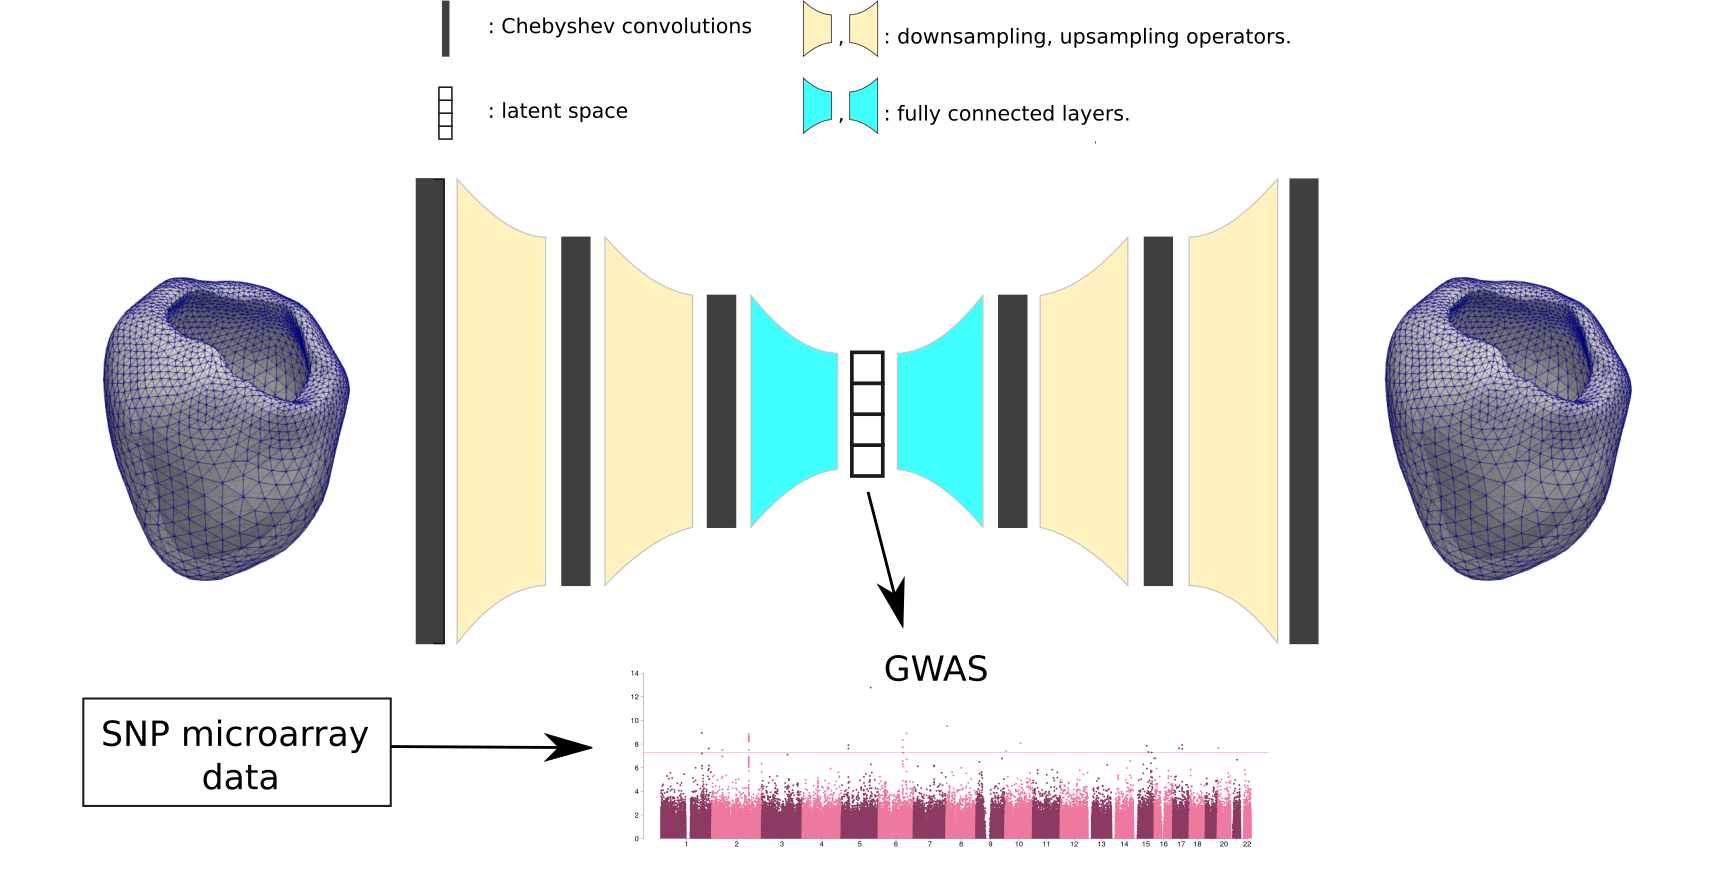
\includegraphics[width=\textwidth]{figs/flowchart.png}
\caption{Flowchart of the steps performed in this work. First, a graph-convolutional autoencoder is trained and applied to our set of LV meshes to produce low-dimensional representations of these shapes. Then, the components of this representation are tested in a GWAS for association with genetic variants.}
\label{fig:flowchart}
\end{figure*}

The unprecedented amount of linked genetic and cardiac imaging data available within the UK Biobank \cite{ref_ukbb} enables the use unsupervised machine learning techniques to automatically learn a set of features that best describe the morphology of the heart. Atlas-based methods have been proposed to generate 3D meshes representing cardiac anatomy from volumetric images \cite{ref_rahman, ref_zhuang_regis_2O10}. We build on top of these works, leveraging the latest advances in graph-convolutional neural networks (GCNN) \cite{ref_bronstein_geom_DL} to learn low dimensional representations that consider mesh topology. While standard convolutional neural networks operate on domains with an underlying Euclidean or grid-like structure (e.g. images), geometric deep learning generalises convolutions to non-Euclidean domains such as graphs, meshes and manifolds, taking into account their topology and irregular structure. Previous works proposed the use of mesh autoencoders to model the expression space of human face surfaces \cite{ref_coma}. Here we show that such models enable learning anatomical variations from cardiac structures, useful to perform genetic association studies.

In this work, we learn compact and non-linear representations of cardiac anatomy in an unsupervised setting via convolutional mesh autoencoders. We hypothesise that the learned features, due to their ability to explain the shape variability across the population, can identify genetic loci that impact cardiac morphology. We show that such representations can indeed discover novel genetic associations using GWAS, which was not previously possible with traditional handcrafted IDPs such as volume, mass and function indices. 


% \appendix
\section{Methods}
 A schematic overview of the proposed method is presented in Figure \ref{fig:flowchart} . The details of each step are outlined in the following subsections. First, we extract a mesh representation of the anatomical structures. In this case, we extracted 3D meshes representing the LV from CMR images of the UK Biobank database using a fully automatic segmentation method \cite{ref_rahman}. We then learn a low-dimensional representation of the 3D meshes which captures anatomical variations using an encoder-decoder model. All meshes are then projected to this latent space to derive a small number of shape descriptors (or latent variables) for each mesh. These features are finally used in GWAS to discover genetic variants associated with shape patterns. 

\subsection{Description of the data}
The proposed framework can be used to discover novel associations between genetic variations and morphological changes in anatomical structures. In this work, we showcase its potential in the context of cardiac images acquired within the UK Biobank (UKB) project (data accession number \ACCESSIONNUMBER). The UKB is a prospective cohort study that between 2006 and 2010 recruited around half a million volunteers across the United Kingdom, aged 40-69 years old at the time of recruitment \cite{ref_ukbb}. This sample aims to represent the whole UK population. The project collected a vast amount of phenotypic information about its participants, and also linked them to their electronic health records (EHR). The collected data includes, among others, genetic data from single-nucleotide polymorphism (SNP) microarrays for all the individuals, and also CMR data for a subset of them (which currently comprises over 40,000 individuals but is planned to reach 100,000 by 2023). These datasets are described in \cite{ref_ukbb_genetics} and \cite{ref_ukbb_cmr}, respectively.

\subsubsection{CMR data}
The CMR imaging protocol used to obtain the raw imaging data is described in \cite{ref_ukbb_cmr}. 
%\paragraph{Segmentation algorithm.}
We employed an automatic segmentation method \cite{ref_rahman} to segment the LV in the CMR images. This method generates a set of registered 3D meshes, i.e. meshes with the same number of vertices and the same connectivity between them. There is one mesh per subject and per time point. In this work, we only use the LV mesh at end-diastole. The LV mesh for subject $i$, $i=1,...,N$, can then be represented as pairs $(\textbf{S}_i, A)$, where $\textbf{S}_i=\big[\,x_{i1}\,y_{i1}\,z_{i1}\,|\,...\,|\,x_{iM}\,y_{iM}\,z_{iM}\,\big]\in \mathbb{R}^{M\times 3}$ is the shape and $A$ is the adjacency matrix of the mesh. We also define, for convenience, the vectorised form of the shapes $\textbf{s}_i=\big(x_{i1},y_{i1},z_{i1},...,x_{iM},y_{iM},z_{iM}\big)\in \mathbb{R}^{3M}$. The adjacency matrix is such that $A_{jk}=1$ if and only if there is an edge between vertices $j$ and $k$ and $A_{jk}=0$ otherwise. The cardiac meshes also have the property of being triangular, so $A_{jk}=A_{kl}=1\implies A_{jl}=1$ for all vertices $i$, $j$ and $k$.

\subsubsection{Genotype data}
SNP microarray data is available for all the individuals in the UKB cohort. This microarray covers \NCALLS\, genetic variants including SNPs and short insertions and deletions. 
%SNPs are single base-pair changes in the DNA sequence that occur with relatively high frequency in the human genome, and represent the most common form of genetic variation in humans. 
The SNP microarrays used in UKB have been described in \cite{ref_ukbb_genetics}. From these genotyped markers, an augmented set of more than 90 millions variants was imputed. The GWAS was performed across the latter dataset, in particular on the autosomes (chromosomes 1 through 22). % The sex chromosomes (X and Y) require a special treatment and are left for future investigation.

The usual quality control steps on the genetic data were performed. This included filtering out rare variants using a threshold for MAF of 1\% (within the subcohort of \NCMRGBR subjects), Hardy-Weinberg equilibrium $p$-value less than $10^{-5}$ and low imputation information score (less than 0.3). This results in set of \NCMRGBR genetic variants. %high call missingness rates (greater than 10\%). 

%% Should this go here?
% Likewise, individuals with high genotype missingness rates were excluded from the analysis.

%% This explanation is unnecessary in the target journal
% SNPs are typically biallelic, meaning that there are two commonly occurring alleles in the population for that specific base-pair, the most frequent one usually considered as the reference allele. The genotype at each SNP is encoded as 0, 1 or 2 depending on the number of copies (or dosage) of the non-reference allele that the individual carries in his or her maternal and paternal chromosomes. 

\subsection{Unsupervised representation learning for genetic discovery}
\label{results:dimensionality_reduction}
% \missingfigure[figwidth=6cm]{Testing a long text string}
%\paragraph{Mesh pre-processing.} 
Given the set of meshes representing the anatomical structure of interest (LV meshes), the pose-sensitive parameters (translation and rotation) were removed using generalised Procrustes analysis. Moreover, since we are interested in understanding the relation between genetic variation and shape patterns, we performed different experiments to understand the impact of mesh scaling in the resulting associations. We considered two scenarios, with and without scaling the meshes: we will use the nomenclature \{$\textbf{S}_{i}^{\text{unscaled}}\}_{i=1}^{N}$ for the set of meshes that preserve the scale of the original image, whereas the $\textbf{S}_{i}^{\text{scaled}}$ meshes are computed as $\textbf{S}_{i}^{\text{scaled}}/\bar{S}_i$, with $\bar{S}_i=(1/M)\sum_{\ell=1}^{M}(x_{i\ell}^2+y_{i\ell}^2+z_{i\ell}^2)^{\frac{1}{2}}$; however, this superscript will be dropped for convenience until we discuss the results for each case, since what follows is similar for both.

Given a set of 3D shapes $\mathbb{S}=\{\textbf{S}_i\}_{i=1}^{N}$, we derive the mean shape and the shape covariance matrix $\textbf{C}$:

\begin{equation}
\bar{\textbf{S}}=\frac{1}{N}\sum_{i=1}^{N}{\textbf{S}},
\end{equation}

\begin{equation}
\bar{\textbf{s}}=\frac{1}{N}\sum_{i=1}^{N}{\textbf{s}},
\end{equation}

\begin{equation}
\textbf{C}=\frac{1}{N-1}\sum_{i=1}^{N}({\textbf{s}}_i-\bar{\textbf{s}})({\textbf{s}}_i-\bar{\textbf{s}})^t.
\end{equation}

Here we propose to learn a reduced set of features that best describe cardiac shape using convolutional mesh-autoencoders (CoMA). We will compare the proposed approach with the well-known method of principal component analysis (PCA). While in PCA only vectorised 3D point clouds $\textbf{s}_i$ will be provided as input (therefore ignoring the data structure and topology), convolutional mesh-autoencoders leverage topological information about the connectivity between the vertices and allows for learning more powerful non-linear representations. However, both approaches can be thought of as particular cases of the encoder-decoder paradigm.

In such a paradigm, there is a pair of encoding and decoding functions, $E_{\theta}:\mathbb{R}^{3M}\rightarrow\mathbb{R}^{n_z}$ and $D_{\phi}:\mathbb{R}^{n_z}\rightarrow\mathbb{R}^{3M}$ that are parameterised by a set of learnable coefficients $\theta$ and $\phi$, respectively. $n_z\in\mathbb{N}$ is the size of the latent space, and it is usually chosen so that $n_z\ll M$ (hence the dimensionality reduction). 

Optimal parameters $\theta^*$ and $\phi^*$ for reconstruction can be estimated by making the composite function $D_{\phi} \circ E_{\theta}$ as close to the identity function $I$ as possible over the training set $\mathbb{S}_\text{train}\subset\mathbb{S}$, using some reasonable measure of reconstruction error $L_{\text{rec}}$ (examples of which are the $L_1$ norm, the $L_2$ norm or the mean squared error MSE) along with a regularisation term $\Omega$, which will account for additional constraints that we want to impose on the model. That is to say, we want to minimise the following function with respect to $\phi$ and $\theta$: 

\begin{equation}
L(\mathbb{S}_\text{train}|\theta, \phi)=
L_{\text{rec}}(\mathbb{S}_\text{train}|\theta, \phi)+
\beta\Omega(\mathbb{S}_\text{train}|\theta, \phi).
\label{eq_loss_function}
\end{equation}

\noindent where $\beta\in\mathbb{R_{\geq 0}}$ is a weighting coefficient for the regularisation term. $\textbf{z}_i:= E_{\theta^*}  (\textbf{S}_i)\in\mathbb{R}^{n_z}$ would then be a low-dimensional representation of the shape $\textbf{S}_i$, whereas $\hat{\textbf{S}}_i:=\big(D_{\phi^*} \circ E_{\theta^*}\big)(\textbf{S}_i)$ is the associated reconstructed shape.

\subsubsection{Principal component analysis.}
PCA is a standard linear technique for dimensionality reduction \cite{pearson_pca}. In terms of the framework detailed above, it can be obtained by requiring $D$ and $E$ to be linear transformations and using the $L_2$ norm, besides imposing an orthogonality constraint on the latent vectors \cite{goodfellow-et-al-2016}.

The idea is to find a basis of vectors  $\mathcal{B}_{n_z}=\{\textbf{v}_i\}_{i=1}^{n_z}\subset\mathbb{R}^{3M}$
for a fixed $n_z < 3M$, such that the $n_z$-dimensional linear subspace generated by $\mathcal{B}_{n_z}$ captures as much of the data variability as possible. It can be shown that such a basis corresponds to the $n_z$ eigenvectors of  $\textbf{C}$ with the largest eigenvalues; i.e. if $\textbf{C}=U^{t}\Lambda U$ where $\Lambda_{ij}=\delta_{ij}\lambda_i$ and $\lambda_i \geq \lambda_j$ if $i\leq j$, then $\mathcal{B}_{n_z}=\{{U\textbf{e}_i}\}_{i=1}^{n_z}$.
$\delta_{ij}$ is the Kronecker delta, which equals 1 if $i=j$ and 0 otherwise.

\subsubsection{Convolutional mesh autoencoder}
In an autoencoder, both the encoding and decoding functions are feed-forward neural networks.
Inspired by recent works on unsupervised geometric deep learning \cite{ref_coma} for facial meshes, we propose to construct a convolutional mesh-autoencoder which uses spectral convolutions \cite{ref_spectral_graph_conv} to learn non-linear and low-dimensional representations of cardiac mesh structures. Here each layer of the encoder and decoder implements convolution operations parameterised by the graph Laplacian, to leverage information about the local context of each vertex. In order to learn global features, a hierarchical approach is used where each layer of the encoder and decoder implements downsampling and upsampling operations, respectively. 
Since the vertices are not in a rectangular grid, the usual convolution, pooling and unpooling operations defined for such topology (usually employed in image analysis) are not adequate for this task and need to be suitably adapted. There are several methods that have been proposed to do this \cite{ref_bronstein_geom_DL}, which can be mainly classified in two broad groups: spatial or spectral. The approach proposed in this work belongs to the latter category, which relies on expressing the features in the Fourier basis of the graph, as explained below.

\paragraph{Spectral convolutions.} The Laplace-Beltrami operator $\mathcal{L}$ (or, more simply, the Laplacian) of a graph with adjacency matrix $A$ is defined as $\mathcal{L}:=D-A$, where $D$ is the degree matrix, i.e. a diagonal matrix with $D_{ii}:=\sum_{j}A_{ij}$ being the number of edges that connect to vertex $i$. The Fourier basis of the graph can be obtained by diagonalising the Laplace operator, $\mathcal{L}=U^t\Lambda U$. The columns of $U$ constitute the Fourier basis, and the operation of convolution $\star$ for a graph can be defined in the following manner:

\begin{equation}
x\star y :=U(U^tx\odot U^ty),
\end{equation}{}

\noindent where $\odot$ is the element-wise product (also known as Hadamard product), and $x$ and $y$ are arbitrary functions defined over the vertices of the graph. Spectral methods rely on this definition of convolution and differ from one another in the specific filter used. In this work, a parameterisation proposed in \cite{ref_spectral_graph_conv} will be used. 
Said method is based on the Chebyshev family of polynomials $\{T_i\}$. The kernel $g_\xi$ is defined as:

\begin{equation}
g_{\xi}(\mathcal{L})=\sum_{i=1}^{K}\xi_i T_i(\mathcal{L}),
\label{eq_chebyshev_filter}
\end{equation}

\noindent where $K$ is the highest degree of the polynomials considered (in this work $K=6$). Chebyshev polynomials have the advantage of being computable recursively through the relation $T_i(x)=xT_{i-1}(x)-T_{i-2}(x)$ and the base cases $T_1(x)=1$ and $T_2(x)=x$. It is also worth mentioning that the filter described by equation \ref{eq_chebyshev_filter}, despite its spectral formulation, has the characteristic of being local.

\paragraph{Autoencoder.} The downsampling and upsampling operations used in this study were proposed in \cite{ref_coma} based on a surface simplification algorithm proposed in \cite{ref_quadric_error}. These operations are defined before training each layer, using a single template shape. Here we utilise the mean shape $\mathbf{\bar{S}}$ as a template.

In each layer of the encoder, the downsampling operation generates a new triangular mesh (with its corresponding new Laplacian), such that the quadric error is minimised. The upsampling operations are created while performing the downsampling: the coordinates of the decimated vertices with respect to the remaining vertices are stored for each layer. 

The inputs to the autoencoder are the vertex-wise-standardized deviations from the mean shape, in which each coordinate of each vertex of the mesh is divided by its own standard deviation (diagonal elements of $\textbf{C}$). By means of this vertex-wise normalisation we aim to prevent small variations in shape in some regions of the LV meshes to be overshadowed in the loss function by large variations in other regions. %\textcolor{red}{Actually, the input to the network belongs to $\mathbb{R}^{M\times 3}$, i.e. is a matrix where each channel  (column) corresponds to one spatial coordinate, but I need to come up with a good notation for this. The way it's written now makes it look like $\textbf{t}_i\in\mathbb{R}^{3M}$}.

\paragraph{Variational Autoencoder.} A Kullback-Leibler (KL) divergence term was added to encourage statistical independence of the different components of the latent representation, which is expected to improve its interpretability \cite{ref_betavae}. We hypothesise that it will also contribute to producing features with higher heritability, i.e. good candidate phenotypes to perform GWAS on.

To train a model with such a loss function, the framework of variational autoencoder (VAE) is utilised. In this framework, during the training phase the encoder maps the input into a probability distribution instead of a fixed vector. To emphasise this, we will replace the notation $E_\theta(\textbf{S})$ for the encoder network by $q_{\theta}(\textbf{Z}|\textbf{S})$, where $\textbf{Z}$ is now a random variable. During training, for the $j$-th latent variable (with $1\leq z_j\leq n_z$) two quantities are learned, $\mu_j$ and $\sigma_j$, and a realisation $z_j$ of the random variable $Z_j\sim\mathcal{N}(\mu_j, \sigma^2_j)$ is produced and passed through the decoder to generate the output mesh. The aforementioned KL-divergence term is then used to encourage the variational approximate posterior to be a multivariate Gaussian with a diagonal covariance structure. The regularisation term is computed as:

\begin{align}
\begin{split}
\Omega(\mathbb{S}_\text{train}|\theta, \phi)&= \mathbb{E}_{\mathbf{s}\sim\hat{p}_{\text{train}}}\
D_{\text{KL}}\Big(q_{\theta}(\textbf{Z}|\textbf{S})||\mathcal{N}(\mathbf{Z};\mathbf{0}, \mathbb{1}_{n_z})\Big)\\
&=\mathbb{E}_{\mathbf{s}\sim\hat{p}_{\text{train}}}
\frac{-1}{2n_z}\sum_{j=1}^{n_z}\Big(\log\sigma^2_j-\sigma^2_j-\mu^2_j+1\Big)
\label{eq_regularisation}
\end{split}
\end{align}

\noindent where $\mathbb{1}_{n}$ is the $n\times n$ identity matrix, $D_{\text{KL}}(p||q)$ is the Kullback-Leibler divergence between probability distributions $p$ and $q$, and $\hat{p}_{\text{train}}$ is the empirical probability distribution associated to $\mathbb{S}_\text{train}$.
$D_{\text{KL}}(p||q):=\int p(x)\ln{\frac{p(x)}{q(x)}}dp(x)$. The last equality in equation \ref{eq_regularisation} arises
from the formula for the KL divergence between two normal distributions where the second one is also standardised. During testing, the mode of the latent distribution, $\pmb{\mu}(\textbf{S})$, is the latent representation of the shape $\textbf{s}$. In the following, we will rename the weighting coefficient $\beta$ from Equation \ref{eq_loss_function} as $w_{\text{KL}}$ to make it more memorable.

\subsection{GWAS}
According to the traditional GWAS scheme, we tested each genetic variant, $X_i\in\{0,1,2\}$, for association with each latent variable $z_k$ through a univariate linear additive model of genetic effects:

\begin{equation}
z_k = \beta_{ik}X_i+\epsilon_{ik}
\label{eq_gwas}
\end{equation}

\noindent where $\epsilon_{ik}$ is the component not explained by the genotype, assumed to be normally distributed. The null hypothesis tested is that $\beta_{ik}=0$. 

Before GWAS, the phenotypes (i.e. latent variables) were adjusted for a set of covariates: sex, age, height, weight, BMI and diastolic and systolic blood pressure. The reason is that these particular covariates have been found to correlate with traditional cardiac indices, and we wish to correct for non-genetic factors affecting our phenotypes of interest. To do this adjustment, multivariate linear regression on these covariates was performed, then the residues of this regression were rank-inverse-normalized. These inverse-normalised residues are the new phenotypes to be tested in the GWAS. Only individuals with British ancestry were considered for the study, to avoid issues related to population stratification. This produced a sample size of \NCMRGBR individuals.

% The outcome of GWAS is usually represented via the so-called Manhattan plots. In these plots, the horizontal axis corresponds to the genomic position of the SNP, where the different chromosomes are juxtaposed along the axis. The vertical axis measures the strength of the association, usually via $-\log_{10}(p)$, where $p$ is the $p$-value of the association as derived from the linear regression in Equation \ref{eq_gwas}.


\section*{Results}
\subsection*{GWAS on the latent representation}
\label{subsec_GWAS}


The comparison of the outcome of GWAS performed on PCA- and CoMA-derived features reveals that the latter method encounters several significant associations with the genotype; in contrast, PCA, despite its comparable reconstruction performance, yields none. % In other words, CoMA allows extracting phenotypes with some level of heritability. 
CoMA experiments and subsequent GWAS were carried out using scaled and unscaled meshes. In both cases, results obtained with $n_z=8$ (eight latent variables) are reported in the main text. Our results suggest that the Kullback-Leibler regularisation term in the loss function is effective when it comes to obtaining an interpretable low-dimensional representation, by keeping the correlation between different latent variables low. This observation is in line with existing literature which shows how stronger KL divergence terms in VAE architectures help to discover interpretable factorised latent representations of visual concepts \cite{ref_betavae}.

\begin{figure*}[ht!]
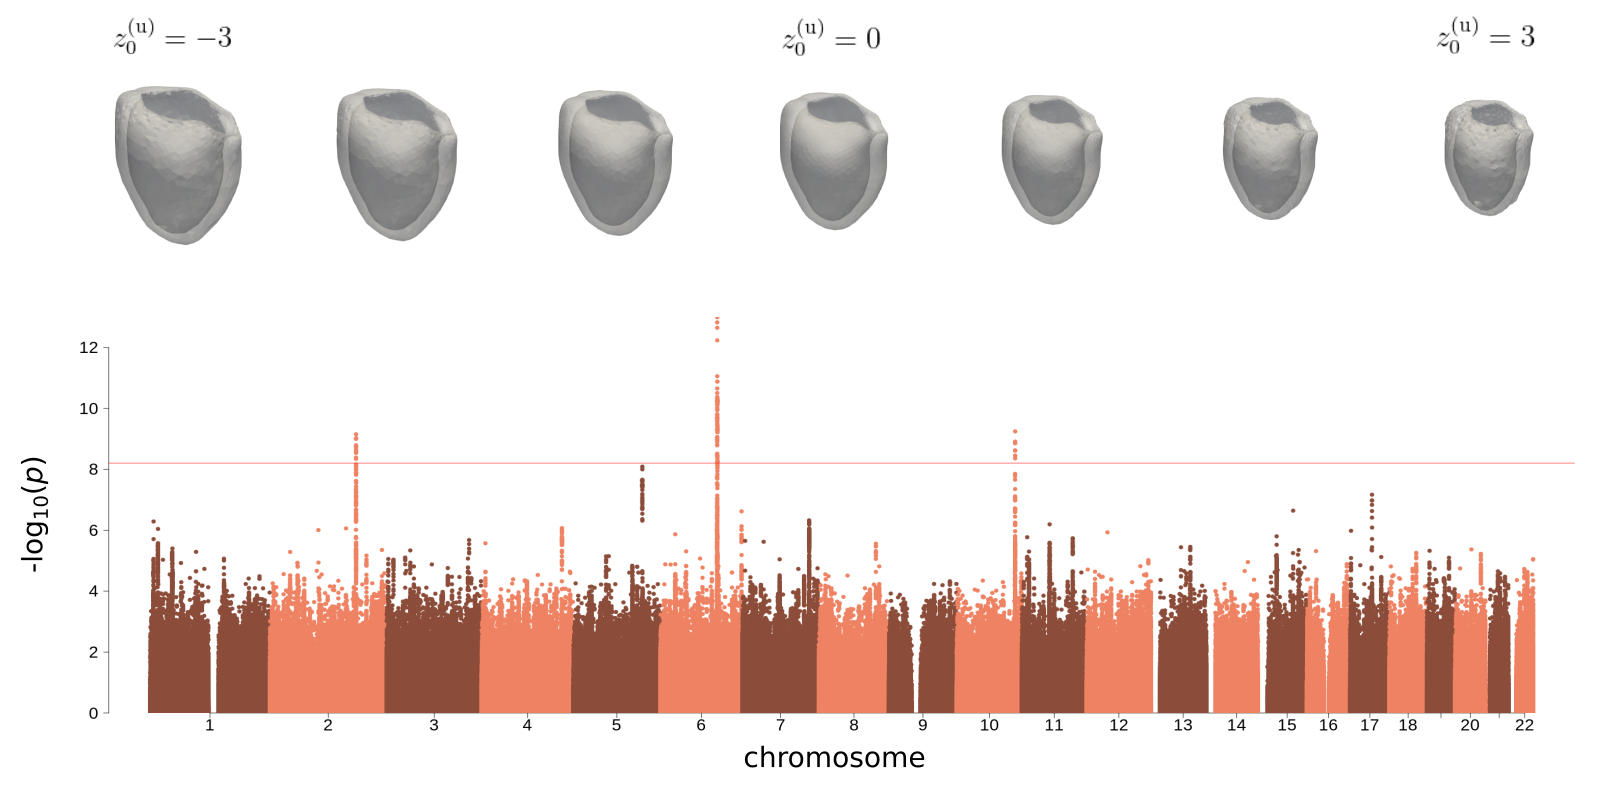
\includegraphics[width=\textwidth]{figs/gwas/GWAS_Experiment2_z0u_unscaled_meshes.png}
\caption{Manhattan plot for LV latent variable $z_0^{(\text{u})}$ along with a set of synthetic LV shapes produced by making $z_i=\lambda \delta_{i1}$ for $\lambda\in\{0, \pm 1, \pm 2, \pm 3\}$. Changes in this variable were found to associate with different LV sizes.}
\label{fig:manhattan_LV_latent_unscaled}
\end{figure*}


% UNSCALED MESHES
For unscaled meshes (i.e. meshes preserving the original scale from the images), several genome-wide significant associations were found, after further adjusting the $p$-value threshold for the number of latent variables tested ($n_z=8$ in this case). Most of these associations belonged to a single latent variable, which we will call $z_0^{(\text{u})}$. The Manhattan plots and synthetic shapes produced by varying $z_0^{(\text{u})}$ around the mean shape are displayed in figure \ref{fig:manhattan_LV_latent_unscaled}. Visual inspection of the effect of varying $z_0^{(\text{u})}$ on the reconstructed LV shape indicates that this latent variable controls the size of the LV. 

In order to further characterise this and the rest of the latent variables found, their Spearman correlation with several cardiac indices was computed. These quantities were derived from the cardiac 3D meshes. Details are explained in the supplementary material. It can be seen that Spearman correlation of LVEDV and $z_0^{(\text{u})}$ is almost perfect.

The locus at chromosome 2 ($p=10^{-10}$) has been reported in  \cite{ref_nayaung, ref_pirruccello} and mapped to gene TTN. This gene encodes for protein titin, which is  responsible  for  the  sarcomere  assembly of the myocytes, which in turn determines stretching, contraction and passive stiffness of the myocardium \cite{granzier_giant_2004}. Therefore, this method, applied to unscaled meshes, allows to retrieve prior knowledge on the genetic basis of LV size.

For scaled meshes, Spearman correlation of latent variables with demographic data was computed and is displayed in figure \ref{fig:relation_to_demographic}.
Interestingly, for scaled meshes, latent variable $z_1^{(s)}$ is significantly correlated with DBP, SBP, BMI and sex (but not with height), whereas latent variable $z_5$ (linked with PLN) is not strongly linked with any demographic variable.
A $t$-test was conducted to determine whether the latent variables were significantly different for subjects with specific cardiac diseases, as compared to people without such diagnoses. To do this, ICD10 codes provided by the UK Biobank were used. The results are presented in \ref{fig:health_outcomes}.

% SCALED MESHES

Variational CoMA yielded a latent variable, which we will call $z_0^{(\text{s})}$, with a single Bonferroni-significant genetic locus in chromosome 6 ($p=10^{-17}$). The associated Manhattan plots are shown in figure \ref{fig:manhattan_LV_latent}, along with the corresponding change in shape produced by the latent variable tested. The morphological impact of $z_0^{(\text{s})}$ is associated with LV sphericity index, as can be seen both by visual inspection of \ref{fig:manhattan_LV_latent} and from the Spearman correlation coefficient in figure \ref{fig:relation_to_indices}.

%(sarco/endoplasmic reticulum Ca$^{2+}$-ATPase)which transports calcium from the cytosol into the SR1. 
%In its dephosphorylated state, PLN lowers the affinity of SERCA for Ca$^{2+}$, thereby inhibiting calcium uptake. Phosphorylation of PLN at serine 16 by PKA (protein kinase A) or threonine 17 by CaMKII (Ca$^{2+}$/calmodulin-dependent protein kinase II) relieves PLN-mediated inhibition of SERCA, thereby increasing SERCA activity and subsequent uptake of calcium. 
Again, we have been able to map this genetic association to gene PLN (phospholamban) with high confidence, based on the literature on genetics of cardiac phenotypes. 
PLN plays a crucial role in cardiomyocyte calcium handling by acting as a primary regulator of the SERCA protein (sarco/endoplasmic reticulum Ca$^{2+}$-ATPase), which transports calcium from the cytosol into the SR1. In its dephosphorylated state, PLN lowers the affinity of SERCA for Ca$^{2+}$, thereby inhibiting calcium uptake by the sarcoendoplasmic reticulum. Phosphorylation of PLN at serine 16 by PKA (protein kinase A) or threonine 17 by CaMKII (Ca$^{2+}$/calmodulin-dependent protein kinase II) relieves PLN-mediated inhibition of SERCA, thereby increasing SERCA activity and subsequent uptake of calcium. The PLN-SERCA interaction is essential for contraction and relaxation of the heart, and is under the regulation of the $\beta$-adrenergic receptor pathway to adapt cardiac output to physiological needs. \cite{maclennan_2003}

\begin{figure*}[ht!]
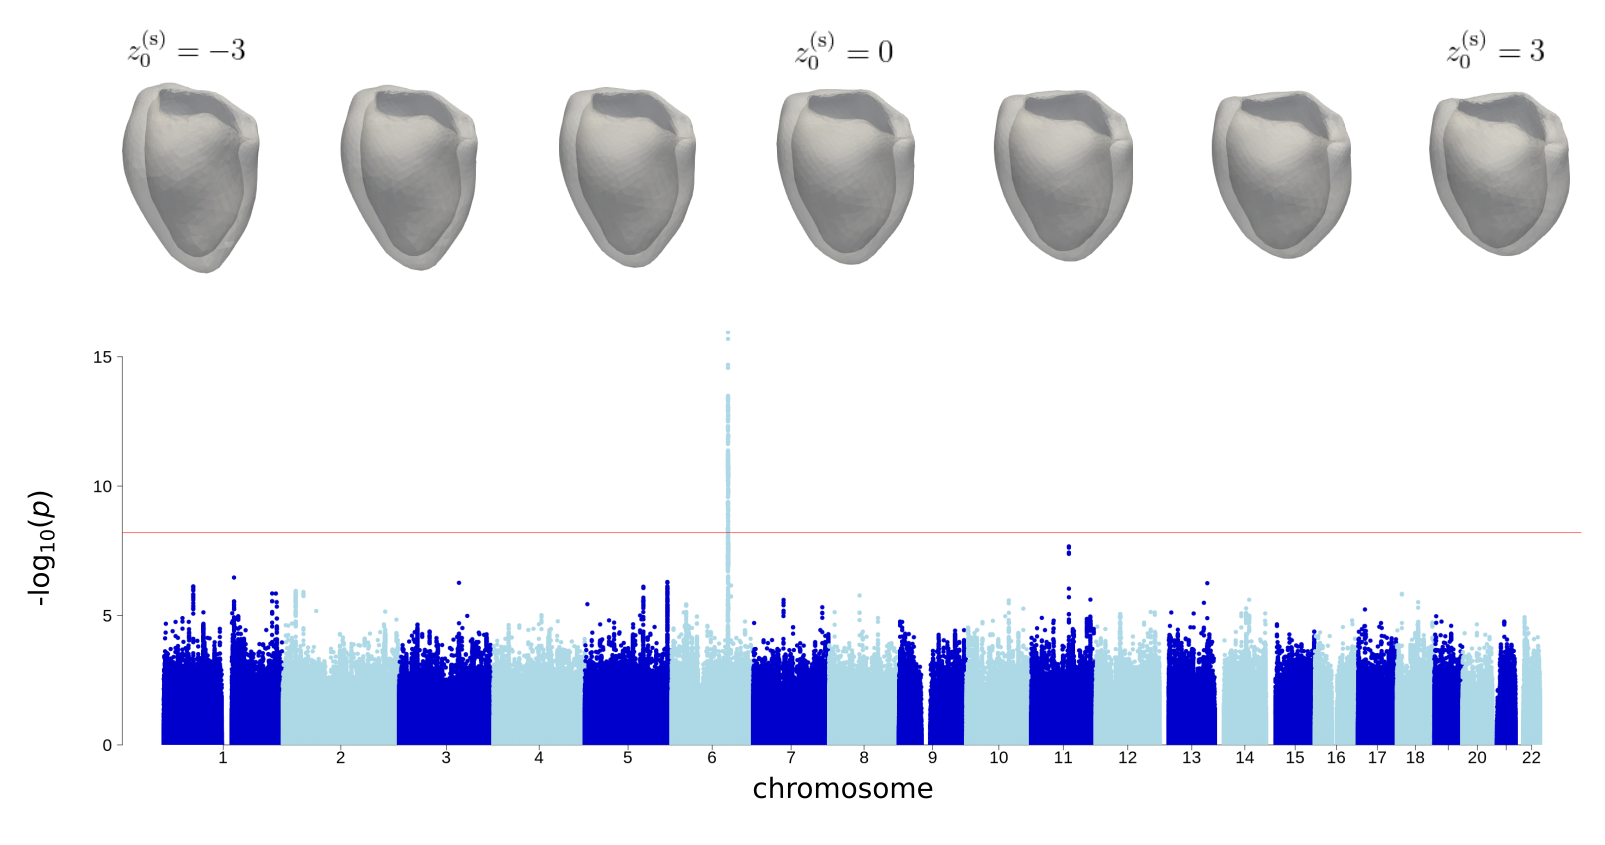
\includegraphics[width=\textwidth]{figs/gwas/GWAS_Experiment1_z0s_scaled_meshes.png}
\caption{Manhattan plot for LV latent variable $z_0^{(\text{s})}$ along with a set of synthetic LV shapes produced by making $z_i=\lambda \delta_{i0}$ for $\lambda\in\{0, \pm 1, \pm 2, \pm 3\}$. This latent variable showed to be associated to LV sphericity index.}
\label{fig:manhattan_LV_latent}
\end{figure*}

Mutations in PLN have a well-established relationship with dilated cardiomyopathy (DCM) \cite{ref_Eijgenraam}. Besides two recent studies, also on UKB data, \cite{ref_pirruccello}, to the best of our knowledge this gene had not been reported in a GWAS of non-disease phenotypes. In \cite{ref_pirruccello}, PLN was found to be associated with LV end-diastolic and end-systolic volumes (LVEDV and LVESV). Interestingly, latent variable $z_0^{(\text{s})}$ yielded a $p$-value slightly lower than the associations reported therein ($10^{-16}$ and $10^{-10}$ for LVEDV and LVESV, respectively). Also, the PLN locus was the only association found for $z_0^{(\text{s})}$, whereas for LV volumes the number of independent genome-wide significant associations is much higher. 

The hypothesis that the PLN association with LV volume is actually mediated by a morphological change captured by $z_0^{(\text{s})}$ was tested. In other words, we checked whether the PLN association is driven by a set of individuals for whom LV volume and $z_0^{(\text{s})}$ are collinear. To do this, LV volume was tested in GWAS after being adjusted for $z_0^{(\text{s})}$ as a covariate, however the PLN association remained significant (see supplementary material), suggesting that PLN controls these two phenotypes independently. Consistent with this conclusion, it can be seen that $z_0^{(\text{s})}$ does not correlate with LV size (see \ref{fig:relation_to_indices}).

Also interestingly, the shape variation associated with high positive values of $z_0^{(\text{s})}$ follows the usual cardiac remodelling linked to DCM \cite{ref_dcm}. Despite the low number of DCM cases within our UKB subcohort (21 subjects), conducting a $t$-test on $z_0^{(\text{s})}$ between individuals with a DCM diagnosis and without, showed that the mean of $z_0^{(\text{s})}$ is significantly different between the two groups ($p=10^{-3}$) (see \ref{fig:health_outcomes})

\begin{figure}[ht!]
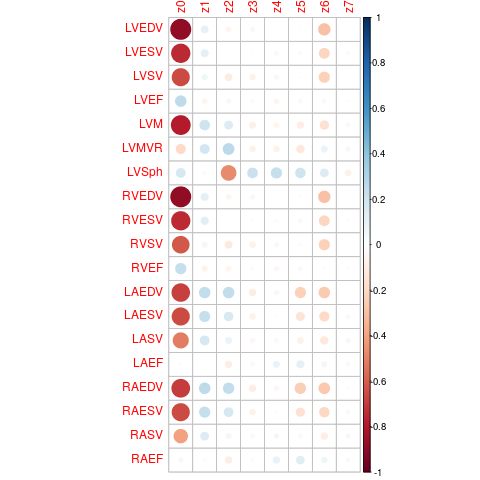
\includegraphics[width=0.5\textwidth]{figs/correlation/experiment_2_vs_cardiac_indices}
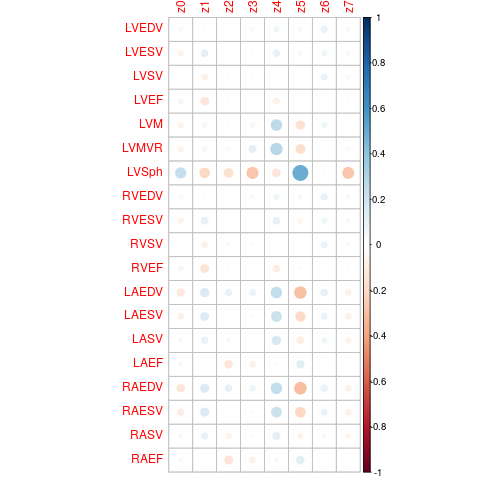
\includegraphics[width=0.5\textwidth]{figs/correlation/experiment_1_vs_cardiac_indices}
\caption{Spearman correlation of the latent variables with traditional cardiac indices for all the cardiac chambers, for CoMA experiments performed on a) unscaled and b) scaled cardiac meshes. XEDV and XESV stand for end-diastolic and end-systolic volume, respectively, whereas $\text{XSV}=\text{XEDV}-\text{XSV}$ and $\text{XEF}=\text{XSV}/\text{XEDV}$ are the stroke volume and the ejection fraction, respectively, where X is one of LV, RV, LA or RA. Finally, LVM stands for LV myocardial mass, whereas $\text{LVMVR}=\text{LVM}/\text{LVEDV}$ is the myorcardial-mass-to-volume ratio and LVSph is LV sphericity index.)}
\label{fig:relation_to_indices}
\end{figure}


\begin{figure}[ht!]
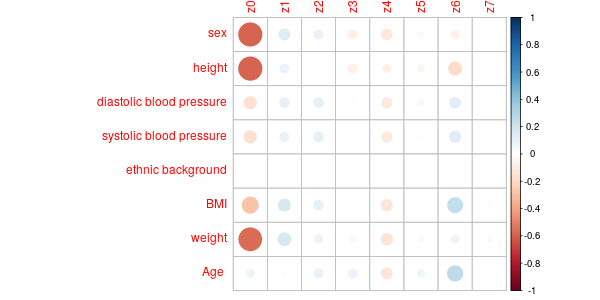
\includegraphics[width=0.5\textwidth]{figs/correlation/experiment_2_vs_demographic_data}
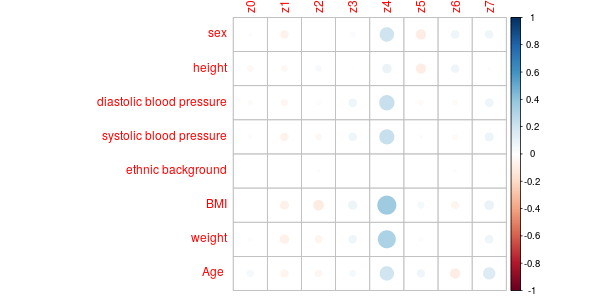
\includegraphics[width=0.5\textwidth]{figs/correlation/experiment_1_vs_demographic_data}
\caption{Spearman correlation of the latent variables with demographic data for all the cardiac chambers, for CoMA experiments performed on a) unscaled and b) scaled cardiac meshes.}
\label{fig:relation_to_demographic}
\end{figure}



%\subsection*{Heritability analysis}
%\textcolor{gray}{Run LD-score regression or GCTA-GREML to estimate heritability of the latent features.}

% \subsection*{Transcriptome-wide associations studies (TWAS)}


\section*{Conclusions}
In this work, we proposed a framework for LV phenotyping based on unsupervised geometric learning techniques on image-derived 3D meshes to discover genetic variations that affect LV shape through GWAS. The proposed methodology is based on finding a latent low-dimensional representation of the CMR-derived LV 3D meshes using convolutional mesh-autoencoders and then performing GWAS on the learned latent features. In contrast with previous efforts carried out to obtain mesh attributes to perform genetic discoveries, we did not look to explictly enforce an association between the phenotype latent representation and the genotype. Instead, we sought to enforce the learning of uncorrelated latent variables, representative of shape characteristics. % This allowed us to assume a uniform distribution of GWAS $p$-values under the null hypothesis of no genetic effect.
As hypothesised, this dimensionality reduction method, using Kullback-Leibler regularisation, yielded phenotypes with significantly associated SNPs. 
Two phenotypes were discovered showing genome-wide significant associations. LV sphericity strongly associated genetic locus mapped to gene PLN. Mutations in this gene have been reported to be a cause for dilated cardiomyopathy. Also, it has been recently reported for the first time to be associated with LV cavity volume, finding that we reproduced in this work. 
These results validate our methodology to extract knowledge about the genetics driving the morphology of organs, leveraging databases that provide linked genetic and imaging data, such as the UKB.


% \section*{Discussion}

% Topical subheadings are allowed. Authors must ensure that their Methods section includes adequate experimental and characterization data necessary for others in the field to reproduce their work.

{\small
\bibliography{gwas_cardiomorpho.bib}
}

% \noindent LaTeX formats citations and references automatically using the bibliography records in your .bib file, which you can edit via the project menu. Use the cite command for an inline citation, e.g.  \cite{Hao:gidmaps:2014}.

% For data citations of datasets uploaded to e.g. \emph{figshare}, please use the \verb|howpublished| option in the bib entry to specify the platform and the link, as in the \verb|Hao:gidmaps:2014| example in the sample bibliography file.

\section*{Acknowledgements}

Acknowledgements should be brief, and should not include thanks to anonymous referees and editors, or effusive comments. Grant or contribution numbers may be acknowledged.

\section*{Author contributions statement}
R.B.,\newline 
N.R.,\newline 
A.S.,\newline 
T.S.M.,\newline 
E.F.,\newline 
A.F.,\newline 
All authors reviewed the manuscript. 

\section*{Additional information}

To include, in this order: \textbf{Accession codes} (where applicable); \textbf{Competing interests} (mandatory statement). 

The corresponding author is responsible for submitting a \href{http://www.nature.com/srep/policies/index.html#competing}{competing interests statement} on behalf of all authors of the paper. This statement must be included in the submitted article file.

% \appendix
\pagebreak
\begin{center}
\textbf{\large Supplemental Materials: Unsupervised deep learning helps disentangle the genetic basis of cardiac morphology}
\end{center}
%%%%%%%%%% Merge with supplemental materials %%%%%%%%%%
%%%%%%%%%% Prefix a "S" to all equations, figures, tables and reset the counter %%%%%%%%%%
\setcounter{equation}{0}
\setcounter{figure}{0}
\setcounter{table}{0}
\setcounter{page}{1}
\makeatletter
\renewcommand{\theequation}{S\arabic{equation}}
\renewcommand{\thefigure}{S\arabic{figure}}
\renewcommand{\bibnumfmt}[1]{[S#1]}
\renewcommand{\citenumfont}[1]{S#1}
%%%%%%%%%% Prefix a "S" to all equations, figures, tables and reset the counter %%%%%%%%%%

\def\code#1{\texttt{#1}} 

\section*{Code and data}
% The code used to produce the results of this paper has been provided in two folders:  \code{CoMA} and \code{GWAS\_pipeline}. The first one contains the code for executing the CoMA experiments, the other contains the code for performing GWAS and generating the associated plots.

The genetic and imaging data used for this work has been downloaded from the UK Biobank (UKB). Since this is protected data for which access must be granted by the UKB, it has not been included in this submission.

% \newline

\section*{Dimensionality reduction and GWAS}

Different dimensions of the latent space $n_z$ and weights $w_{\textrm{KL}}$ were studied, the aim being to achieve a compromise between reconstruction error and interpretability (and hence heritability) of the components.

Figure \ref{fig:pca_vs_coma} shows a comparison of the reconstruction error obtained through PCA and CoMA, as a function of the number of the components $n_z$ of the latent space. CoMA and PCA yield comparable reconstruction errors, with CoMA outperforming the latter slightly. No significant difference was found between non-variational and variational CoMA.
%whereas increasing $w_\text{KL}$ leads to worse quality of the reconstructions, as expected. 
Also, adding the $D_\textrm{KL}$ regularisation term leads to the expected statistical properties of the latent representation of the shapes (independence and isotropy), as can be seen in the supplementary material.

\begin{figure}[ht!]
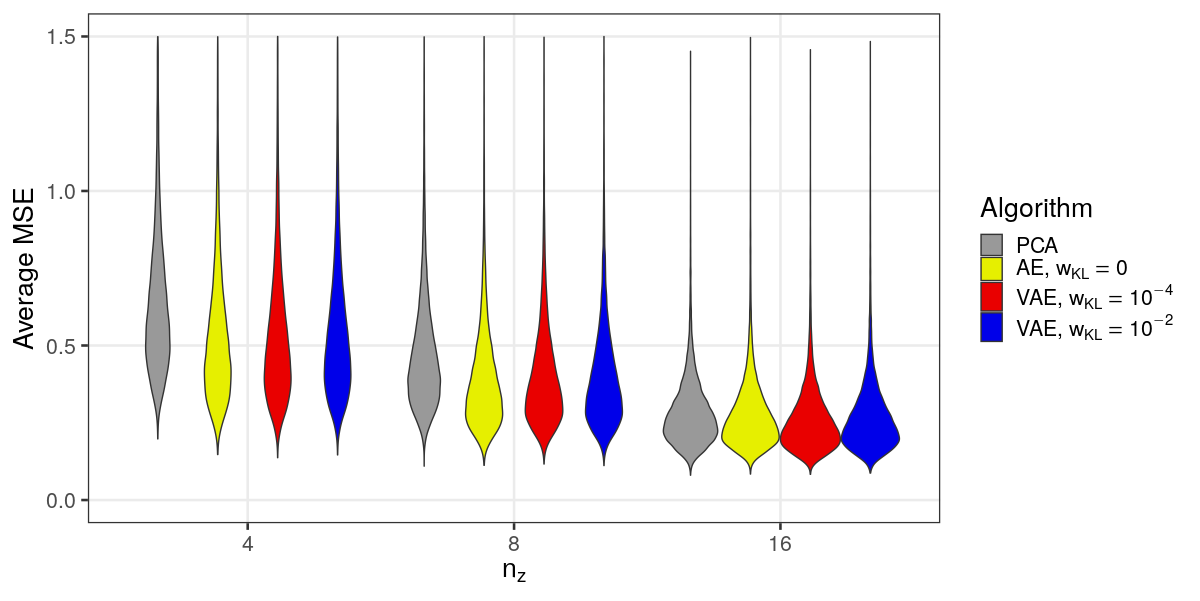
\includegraphics[width=\linewidth]{figs/performance.png}
\caption{Distribution of reconstruction errors (measured as the MSE averaged across the vertices of the mesh) for models trained with different number of components in the latent space, using PCA and CoMA. As a reference, given the vertex-wise normalization that is performed on the meshes, if the real and reconstructed shapes are totally independent the expected value of MSE would be around 2, whereas if we reconstruct the mean shape it would be around 1.}
\label{fig:pca_vs_coma}
\end{figure}

\subsection*{Implementation details}
For the autoencoder, we ran a grid optimisation scheme for meta-parameter selection, both for the architecture and the learning process. For each number of components $n_z$ and regularisation weight $w_\textrm{KL}$, the execution that presented the minimum mean squared error (MSE) within the validation set was chosen.
The autoencoder architecture is explained in table \ref{table:AE_arch}. After each convolutional layer, a ReLU activation function was applied. The number of samples used for training was 5,000, whereas the validation set contained 1,000 individuals. Adam optimiser was used to find optimal network parameters, by minimising the MSE reconstruction loss.

\begin{table}
\begin{center}
\begin{tabular}{|c|c|c|}
\hline
          & \textbf{Input} & \textbf{Output} \\ \hline
ChebConv  & $2677\times 3$ &  $2677\times 16$ \\ \hline
DS        & $2677\times 16$ & $670\times 16$ \\ \hline
ChebConv  & $670\times 16$ & $670\times 16$ \\ \hline
DS        & $670\times 16$ & $168\times 16$ \\ \hline
ChebConv  & $168\times 16$ & $168\times 16$ \\ \hline
DS        & $168\times 16$ & $56\times 16$\\ \hline
ChebConv  & $56\times 16$ &  $56\times 32$\\ \hline
DS        & $56\times 32$ &  $28\times 32$\\ \hline
ChebConv  & $28\times 32$ &  $28\times 32$\\ \hline
FC        & $28\times 32$ &  $8\times 1$\\ \hline
\end{tabular}
\end{center}
\caption{Architecture of the encoder part used for each of the cardiac chambers. The decoder has the same architecture but reading from the bottom upwards and inverting input and output. (ChebConv: Chebyshev convolution, DS: downsampling, FC: fully connected layer.)}
\label{table:AE_arch}
\end{table}

The network training was performed on MULTI-X, our middleware software platform to distribute the computational load on Amazon Web Services EC2 virtual machines (in particular P2 instances with NVidia Tesla K80 GPUs), and using on-premise computational resources endowed with NVidia Tesla M60 GPUs. The code used to generate these results is publicly available at \url{www.github.com/rbonazzola/cardiac\_coma} % \textcolor{red}{The current URL is \url{www.github.com/rbonazzola/pytorch\_coma/tree/cardiac\_develop}.

\subsection{Statistical properties of the latent variables}

Figure \ref{fig:z_distribution} shows the distribution of the latent variables produced by the VAE experiment on scaled meshes and presented in the main text. As stated there, these results show that, as expected, the variables are isotropic and statistically independent.

\begin{figure}
 \centering
 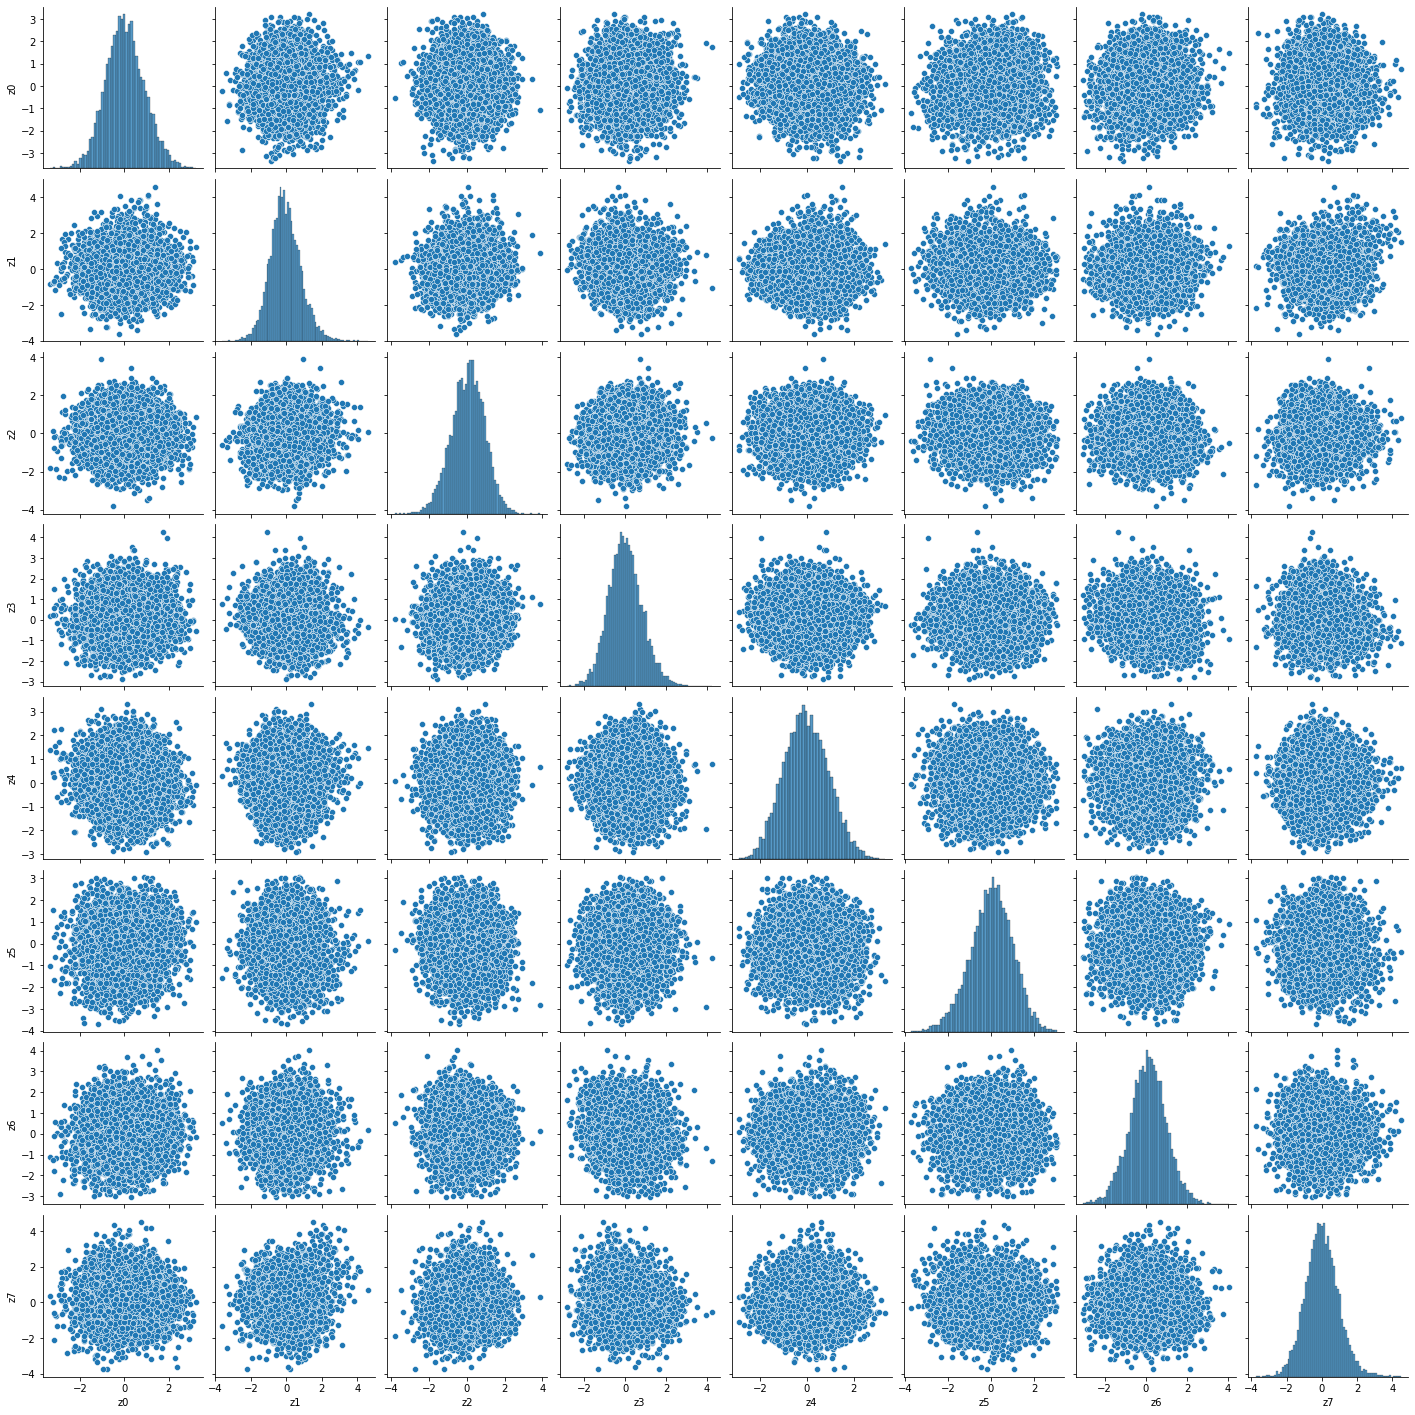
\includegraphics[width=\textwidth]{figs/supplementary/z_distribution.png}
 \caption{Distribution of the 8 latent variables for the experiment on unscaled meshes whose results are presented in the main text.}
 \label{fig:z_distribution}
\end{figure}

\subsection{Interpretation of the latent variables.} An interpretation of the impact of each of the components of the latent basis on LV morphology was achieved by varying the components of the latent space one at a time (while keeping the rest fixed at zero) and generating the associated synthetic shapes by means of the trained decoder. % heat map showing the deviations from the mean shape. 
In the main text of this paper, only those components that yielded Bonferroni-significant SNP associations are shown, along with the corresponding Manhattan plots. The rest of them are included in this supplementary material.

\begin{figure}
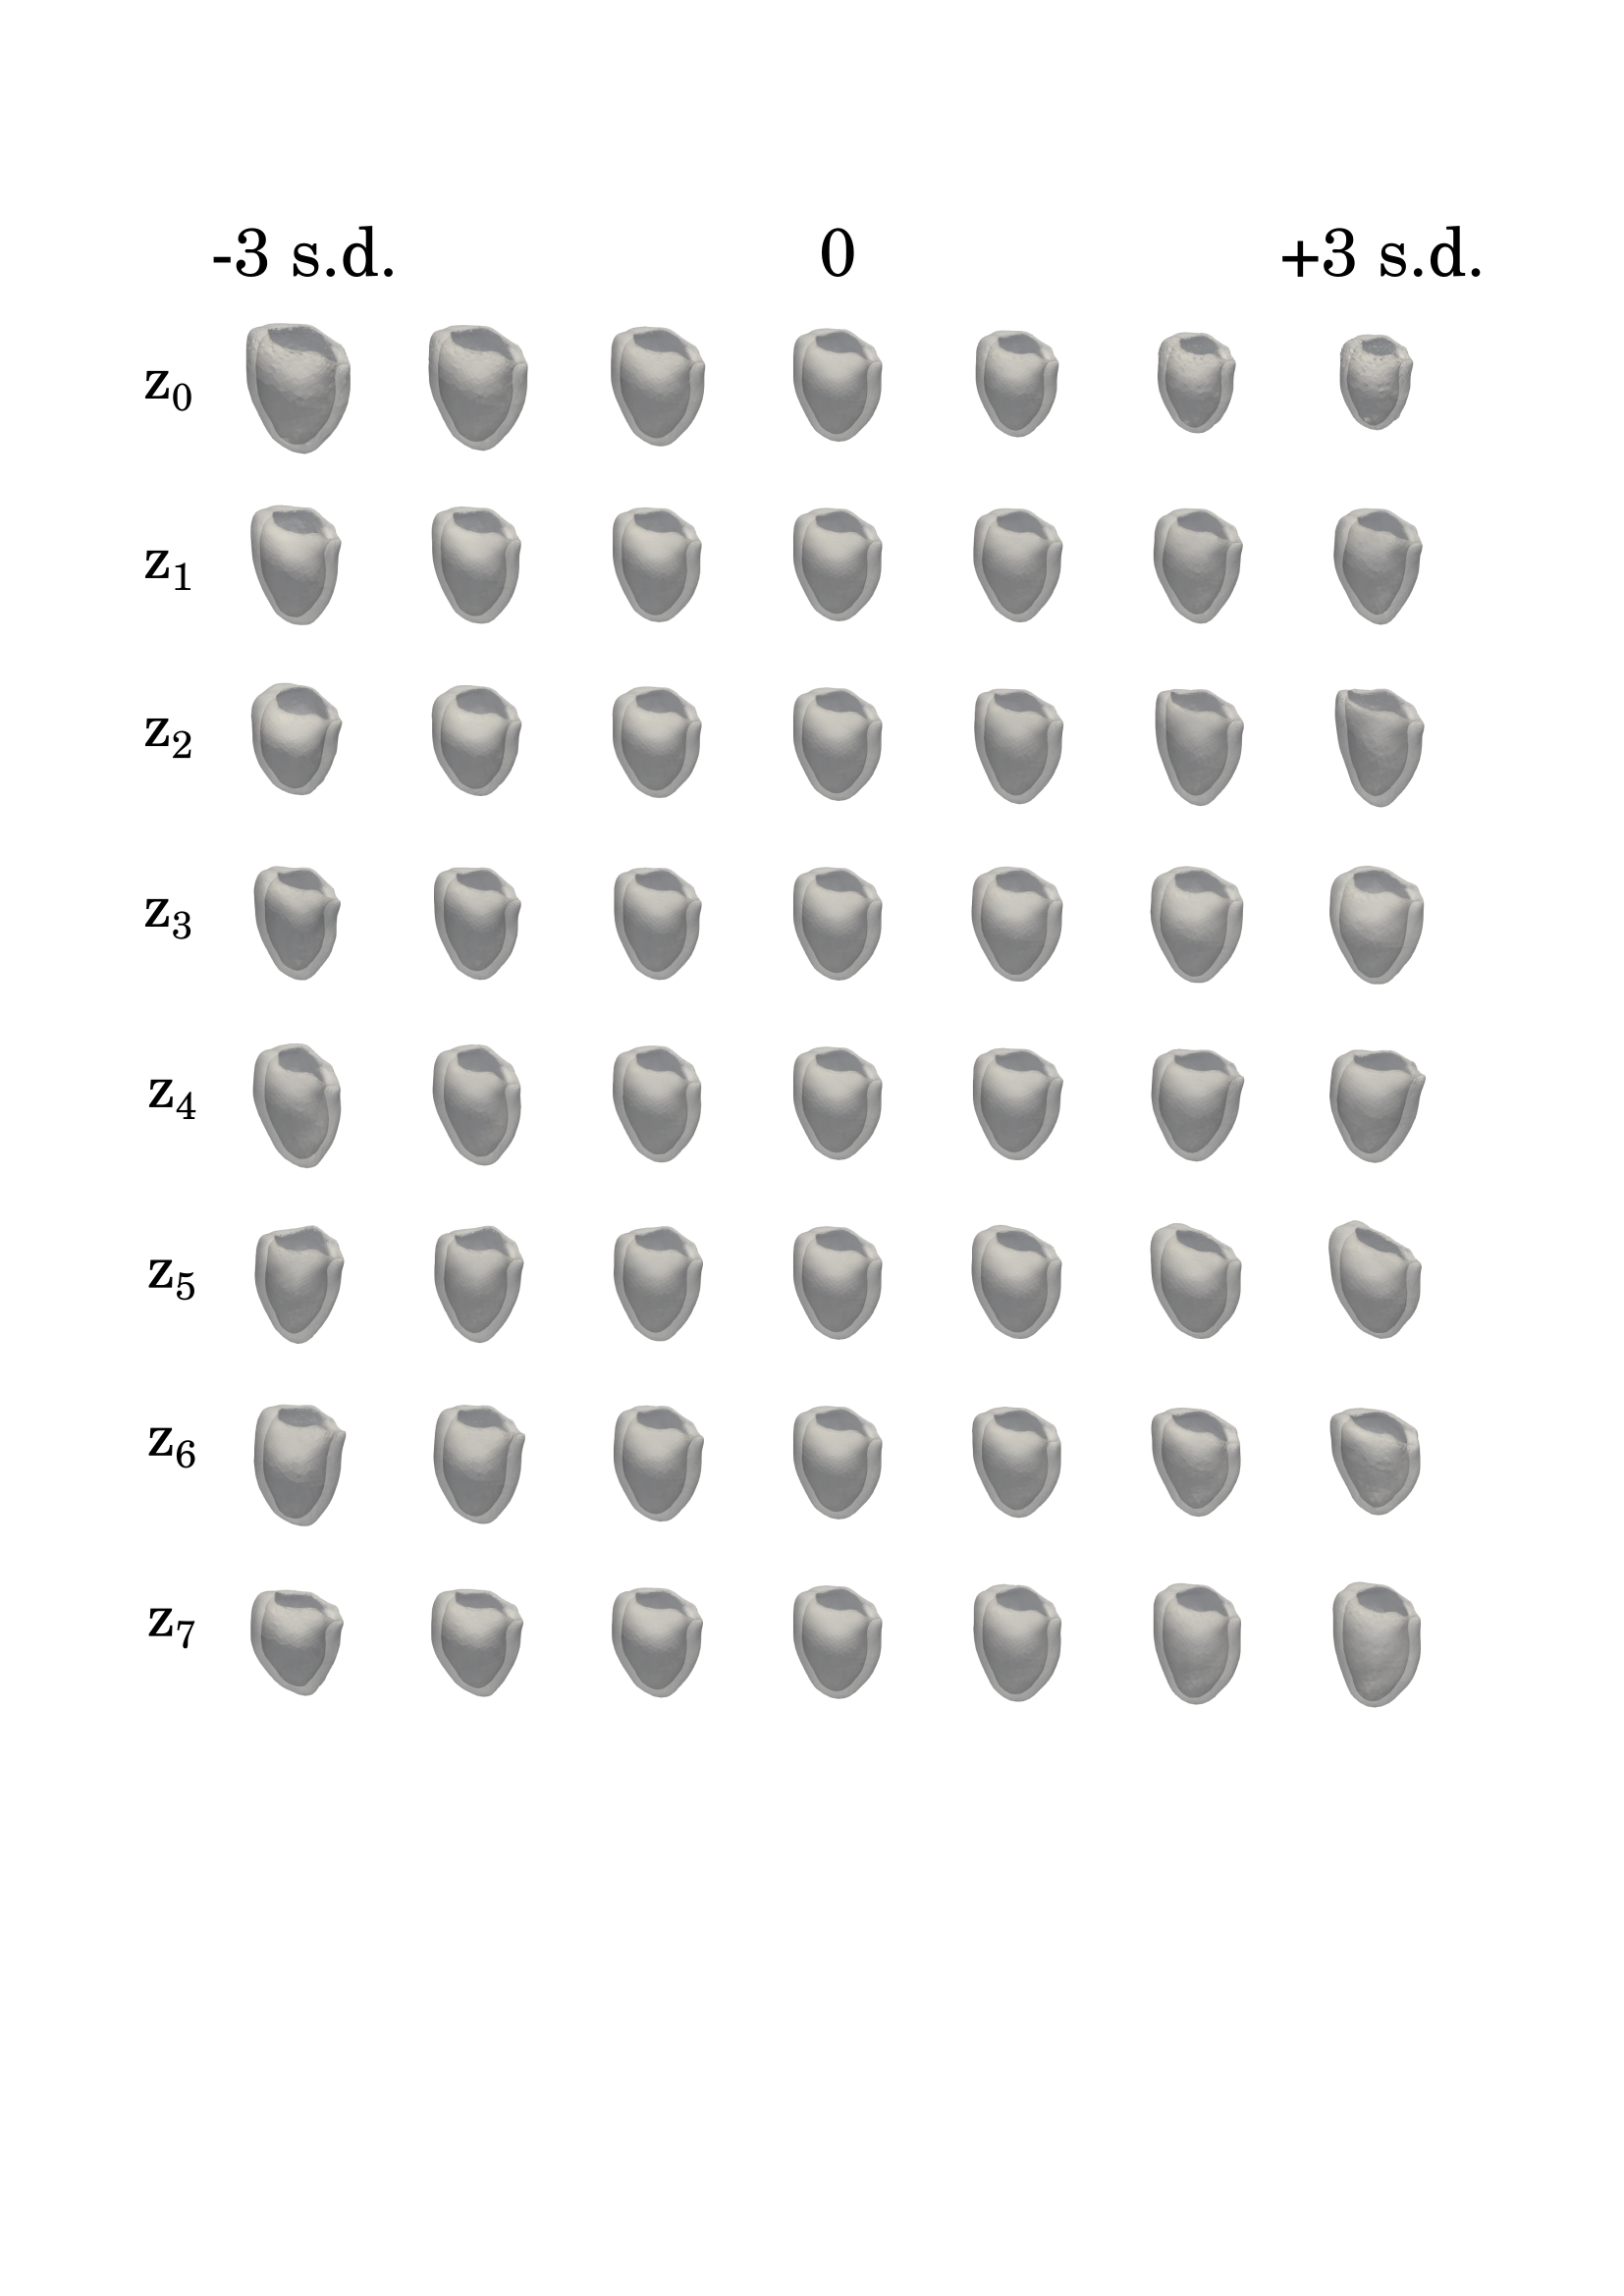
\includegraphics[width=\textwidth]{figs/supplementary/experiment_2_synthetic_meshes}
\caption{Effect of each latent variable on LV morphology, for CoMA experiment performed on unscaled meshes.}
\label{fig:experiment_2_synthetic_meshes}
\end{figure}

\begin{figure}
\includegraphics[width=\textwidth]{figs/supplementary/experiment_1_synthetic_meshes}
\caption{Effect of each latent variable on LV morphology, for CoMA experiment performed on scaled meshes.}
\label{fig:experiment_1_synthetic_meshes}
\end{figure}


\subsection*{Relation with other variables}
\textbf{Sphericity}: sphericity index was calculated as follows: first, the convex hull of each cardiac mesh was obtained, and then its surface area $A_{\text{CH}}$ and volume $V_{\text{CH}}$ of the convex hull. The sphericity was obtained as $\text{Sph}=(36\pi V_{\text{CH}})^{2/3}$, which is tantamount to the inverse of the ratio of $A_{\text{CH}}$ and the surface area of a sphere with volume $V_{\text{CH}}$.

\begin{figure}
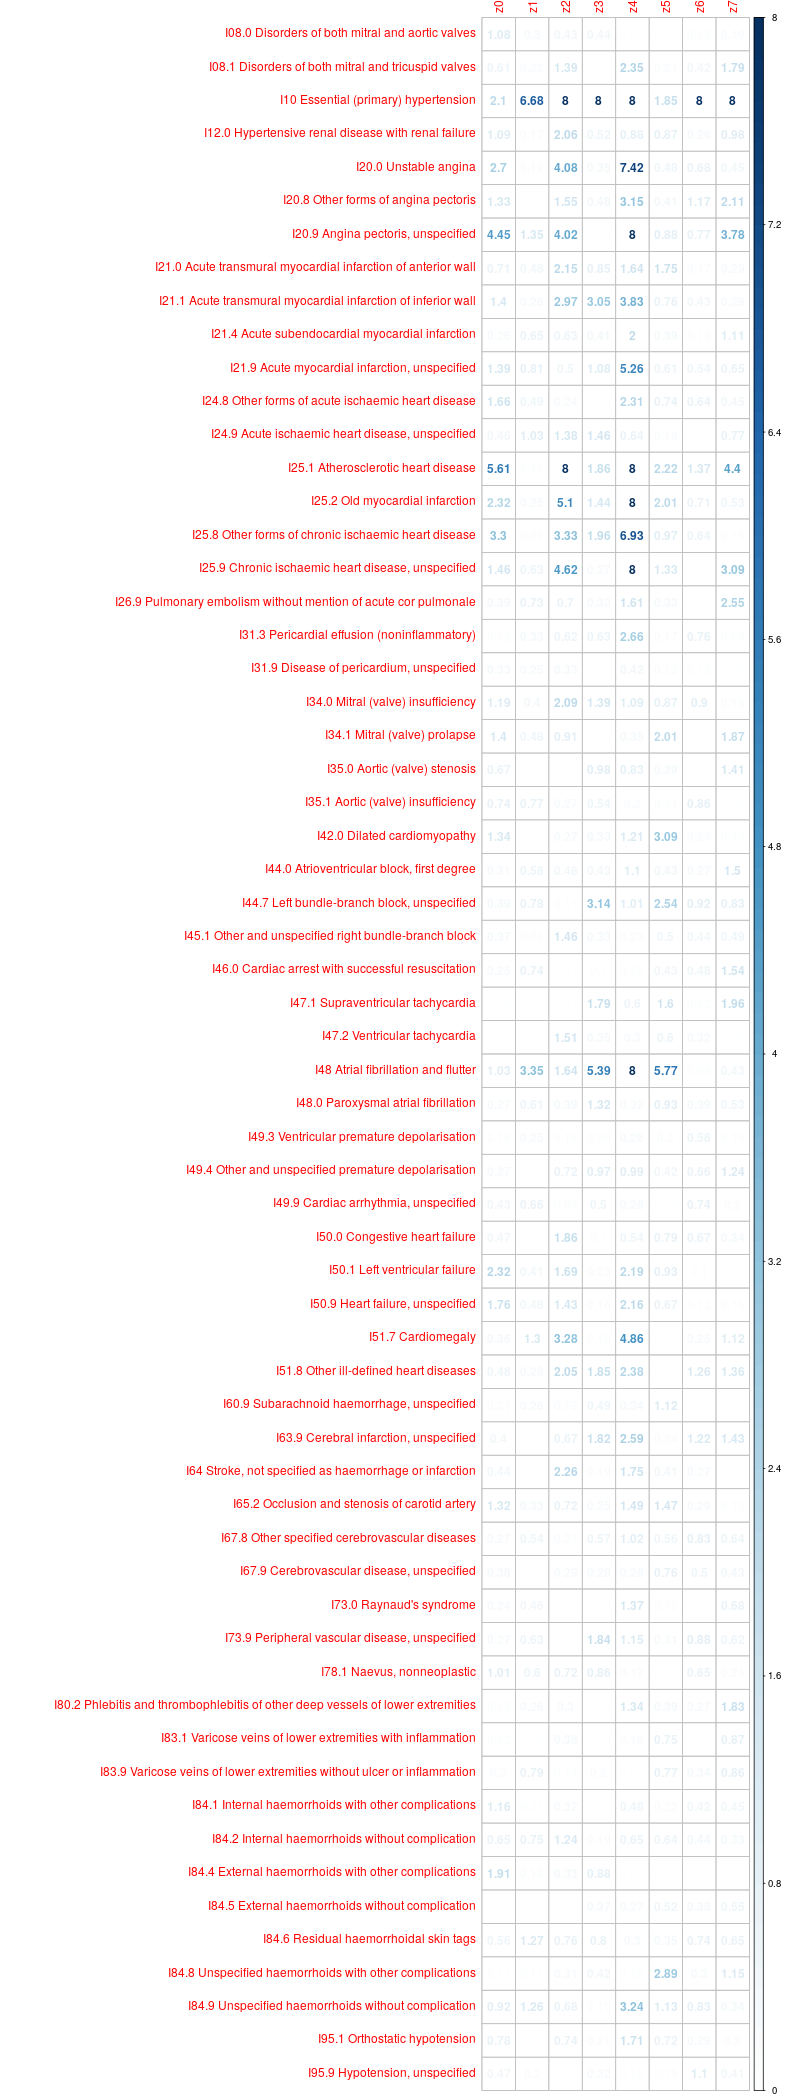
\includegraphics[width=0.5\textwidth]{figs/diseases/experiment_1_health_outcome_t-test}
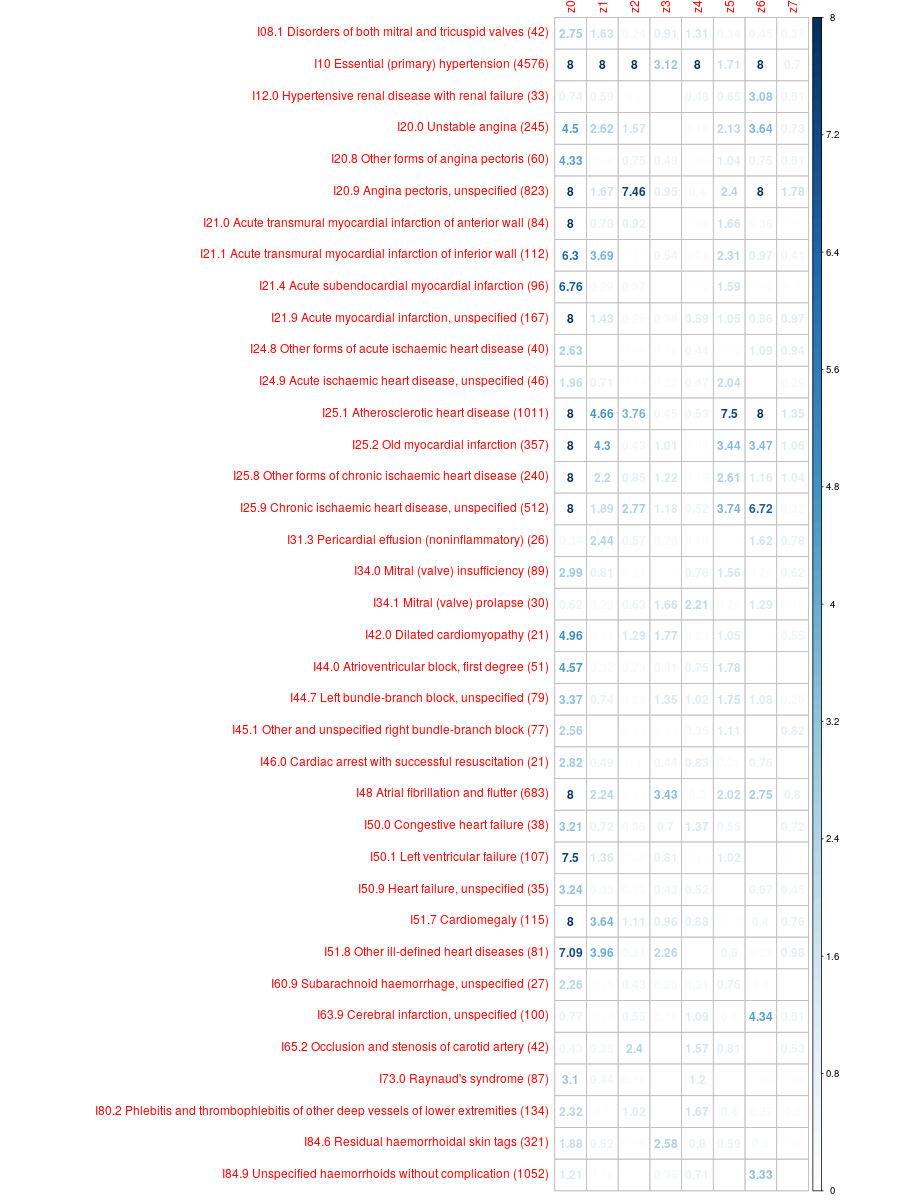
\includegraphics[width=0.5\textwidth]{figs/diseases/experiment_2_health_outcome_t-test}
\caption{$-\log_{10}(p)$ for the $t$-tests of the latent variables on different health outcomes provided by the UK Biobank. $p$-values lower than $10^{-8}$ have been thresholded to $10^{-8}$.}
\label{fig:health_outcomes}
\end{figure}

\subsection{GWAS}

\subsubsection{GWAS on adjusted LVEDV}
\textcolor{purple}{LV volume was tested in GWAS after being adjusted for $z_0$, however the PLN association remained significant (see figure \ref{fig:LVEDV_adj_by_z5}), suggesting that PLN controls these phenotypes independently.}

\begin{figure}[ht!]
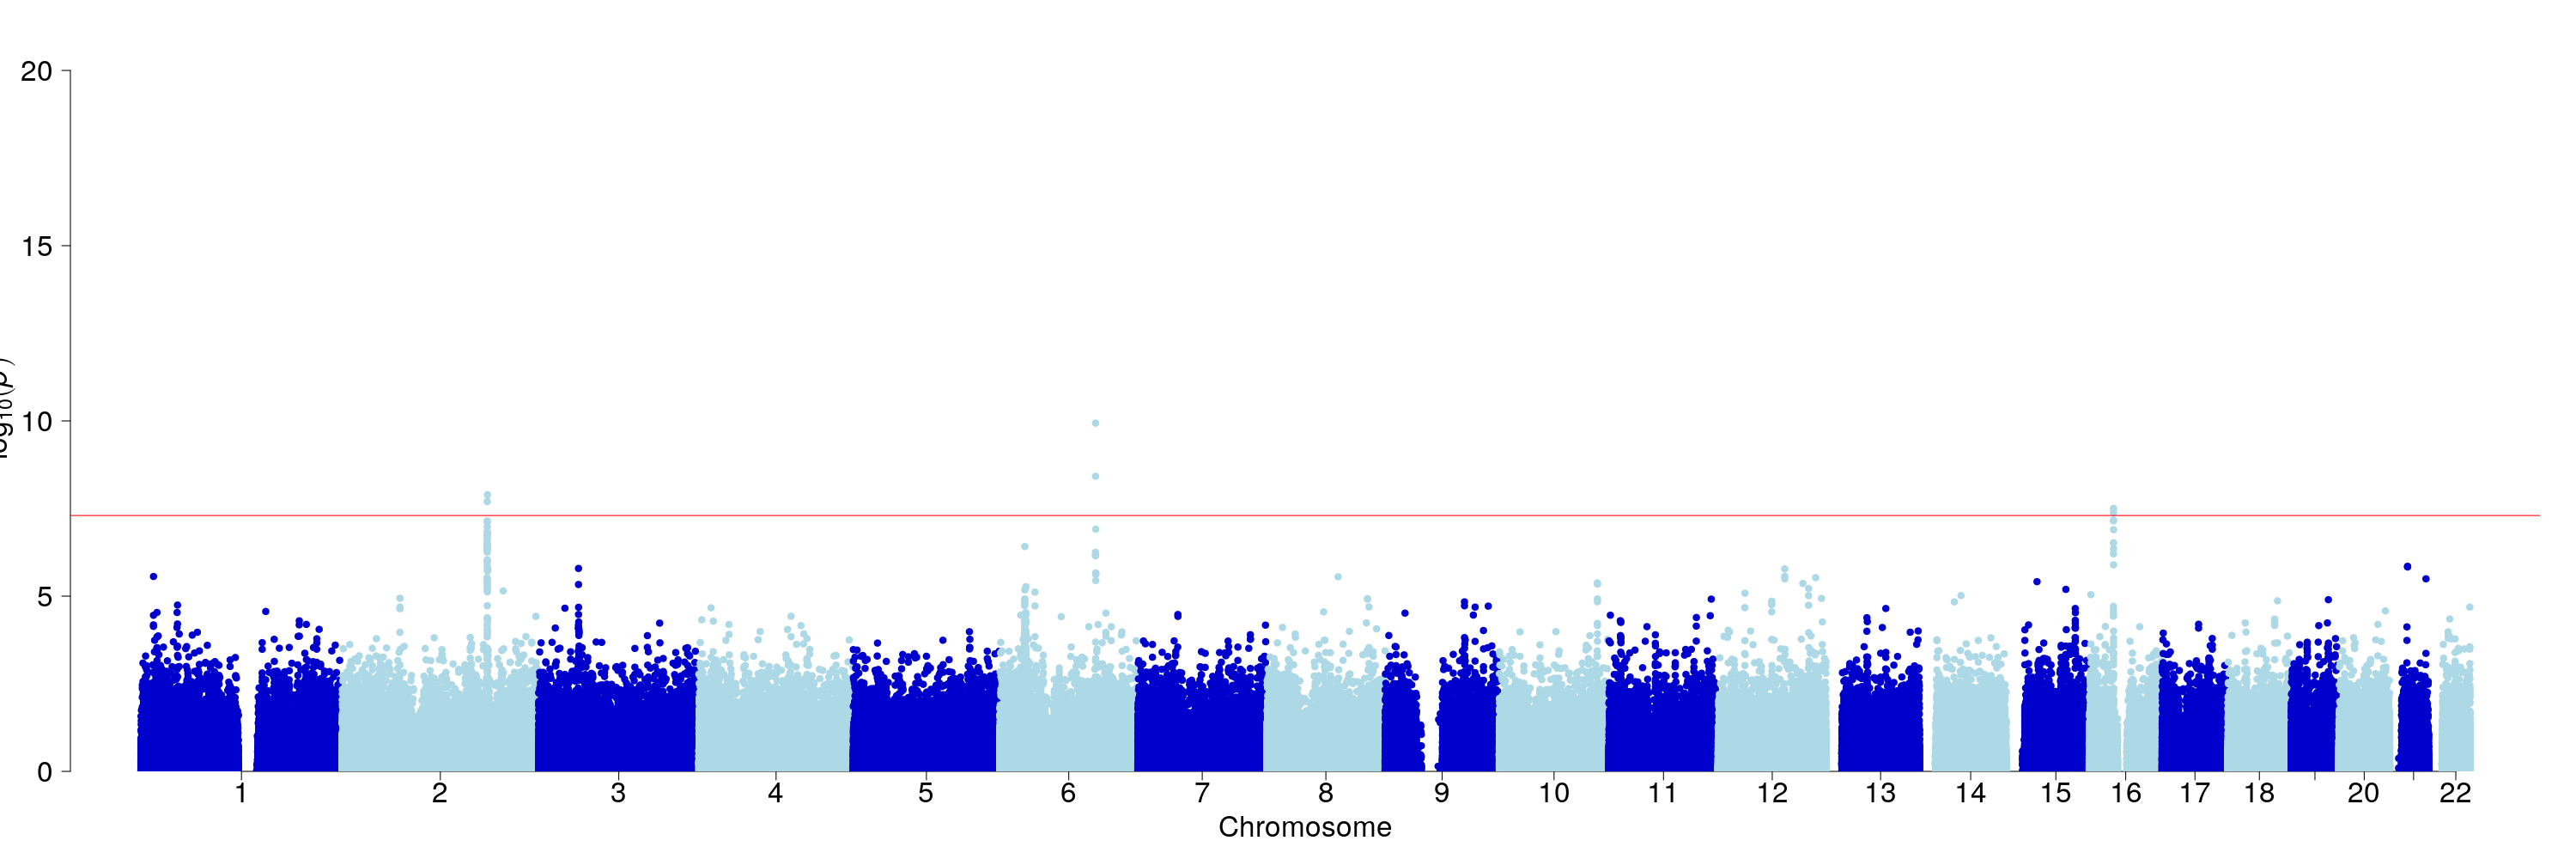
\includegraphics[width=\textwidth]{figs/supplementary/GWAS__LVEDV__std_covariates_adj_by_z5__GBR_ALL__qc__manhattan}
\caption{Manhattan plot showing the outcome on GWAS on LVEDV after adjusting for latent variable $z_0^{(\text{s})}$}
\label{fig:LVEDV_adj_by_z5}
\end{figure}


\subsubsection{Q-Q plots}
In this section, we provide quantile-quantile plots, or Q-Q plots, for the GWAS that yielded significant associations. % For the readers' convenience, we explain how to interpret these plots in the following paragraph. 

% A Q-Q plot is simply a way to compare two frequency distributions, $p_1$ and $p_2$, where $\int p_i(x)dx=1$. If $p_1$ and $p_2$ are continuous distributions, the associated Q-Q plot is built by matching the values that correspond to the same quantiles en each distribution, i.e. the graph is given by $\{(x,y): \int_{-\infty}^xp_1(t)dt=\int_{-\infty}^yp_2(t')dt'\}$
% In this case, it is employed to compare the distribution of $-\log_{10}(p)$ obtained by the GWAS and the same distribution if the $p$-values were uniformly distributed in $[0,1]$, which would be the case if the null hypothesis were true for all the tests. If there is some genetic signal present (i.e. the null hypothesis is rejected for some SNPs), then one should expect a deviation from the identity line. In summary, Q-Q plots provide a convenient way to easily tell whether a GWAS has yielded any significant association.

Figures \ref{fig:qq_scaled} and \ref{fig:qq_unscaled} show the Q-Q plots for the GWAS performed on the latent representations of scaled and unscaled meshes, respectively.

\begin{figure}
 \centering
 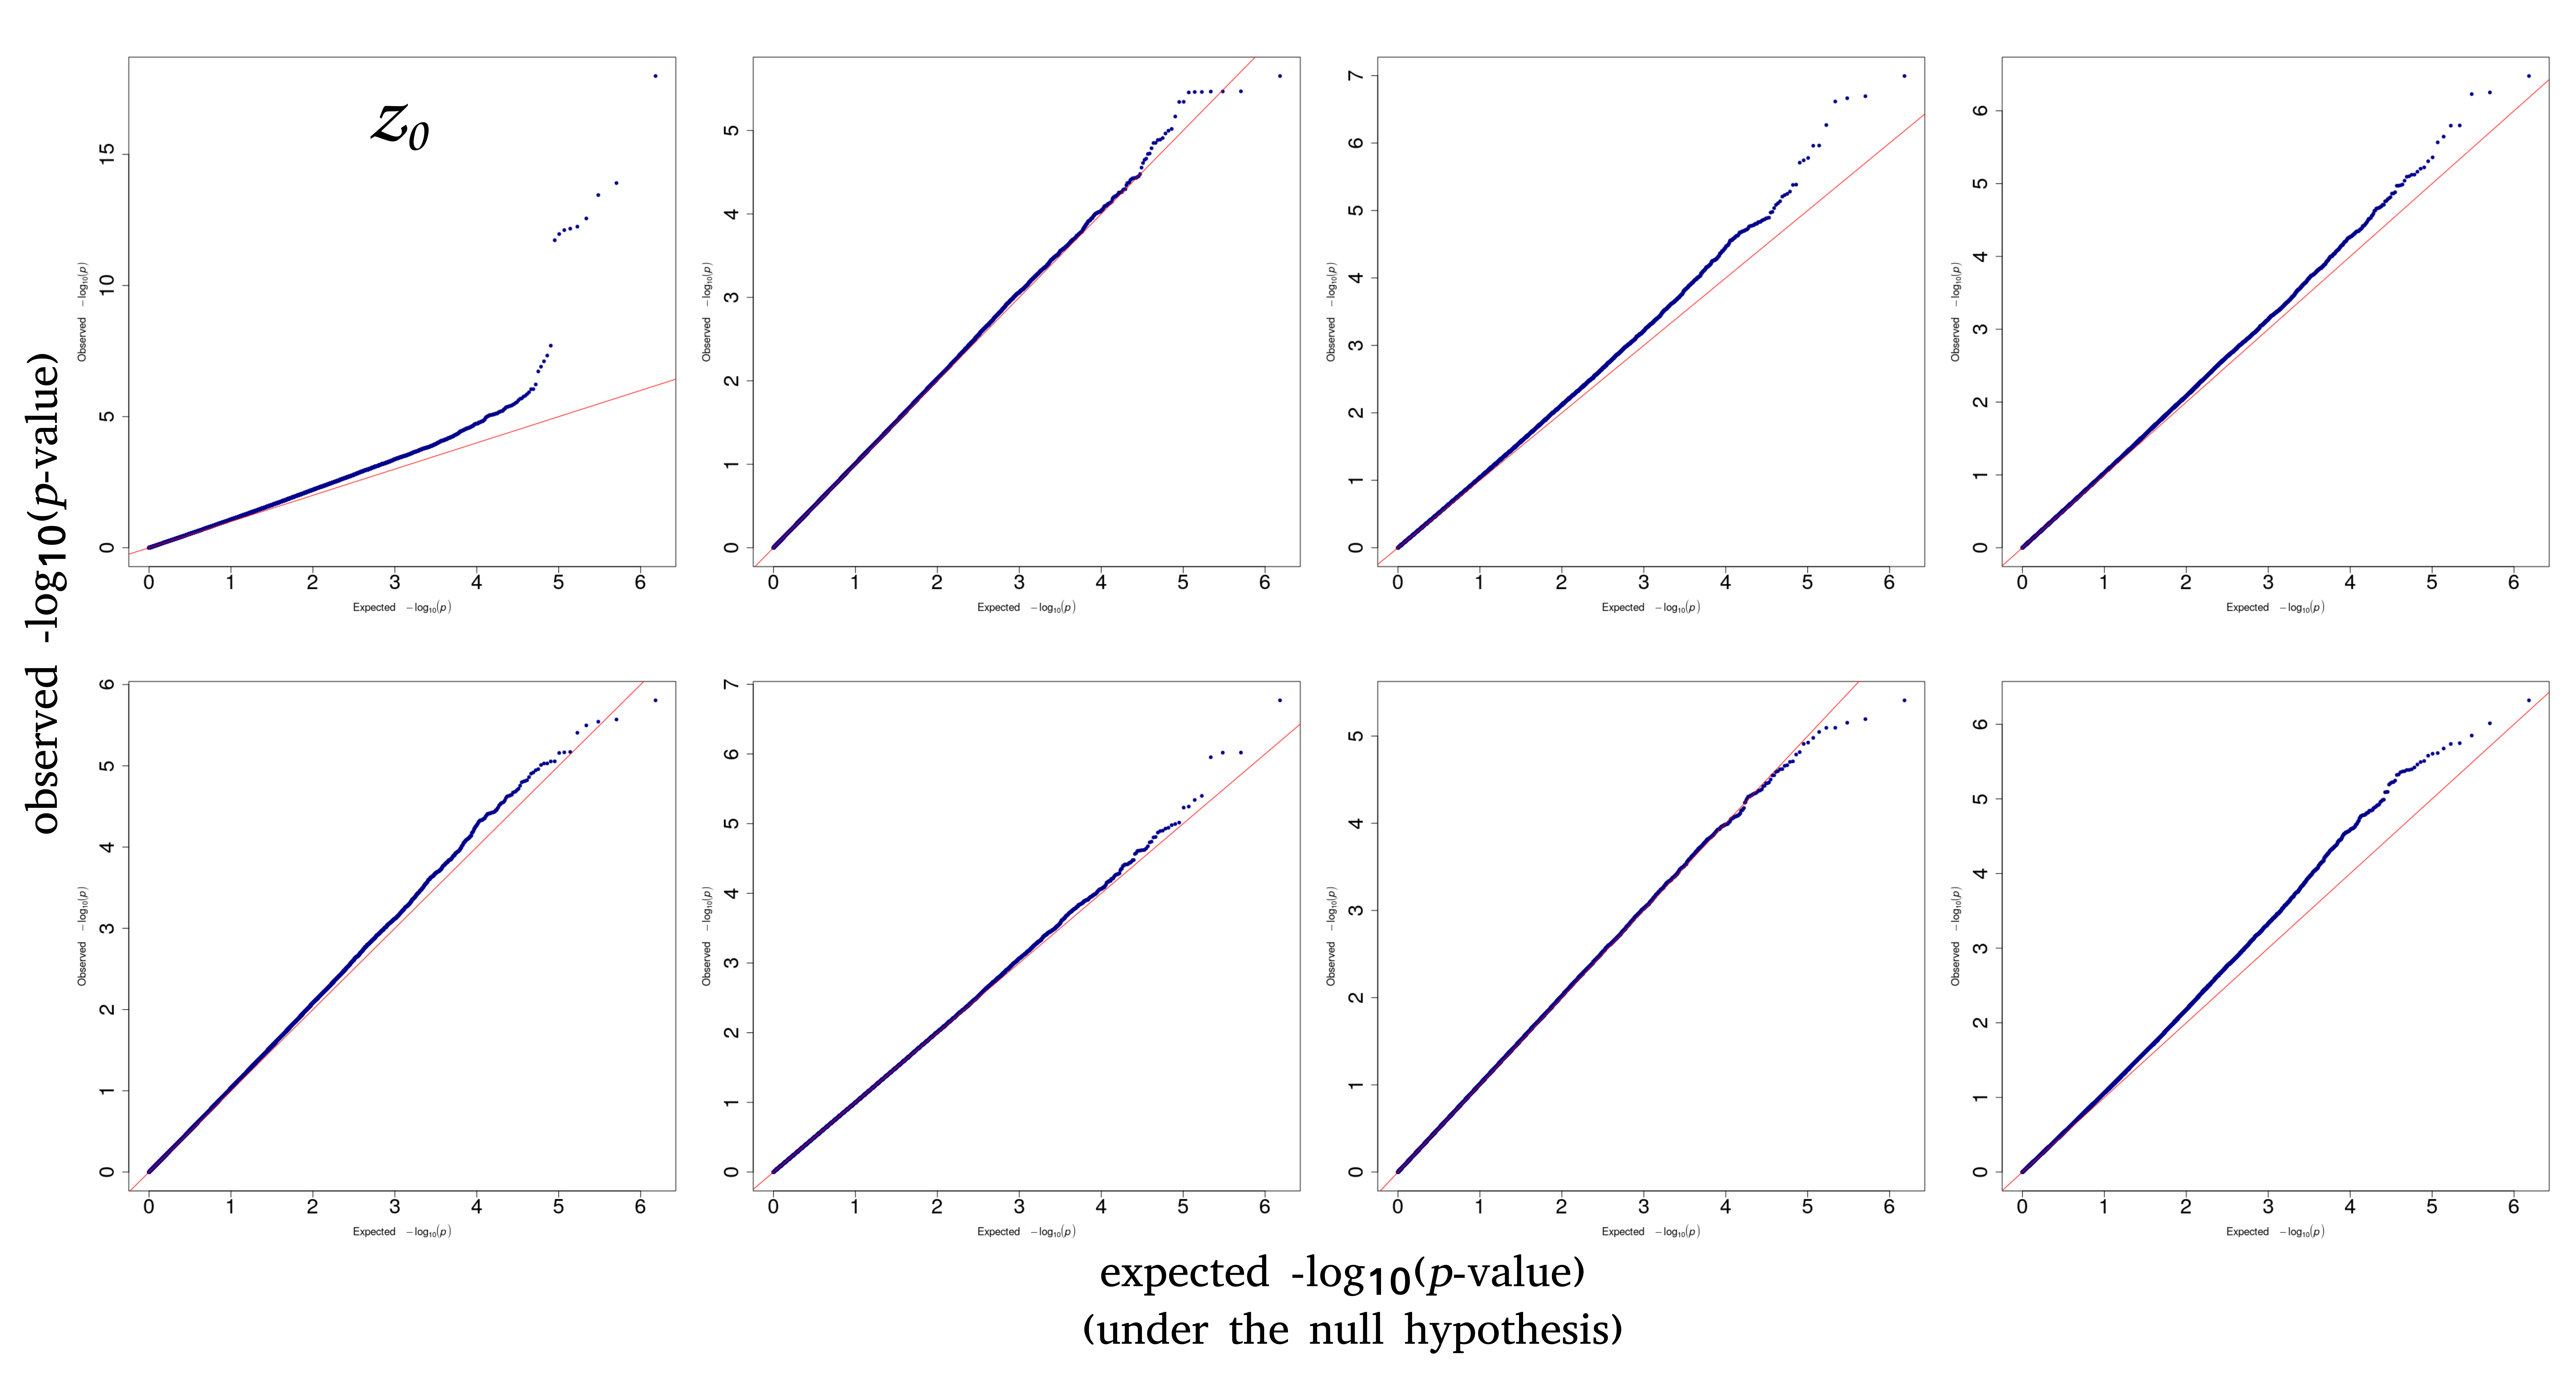
\includegraphics[width=\textwidth]{figs/supplementary/scaled_qq.png}
 \caption{Q-Q plots for the GWAS on each of the 8 latent variables of scaled LV meshes. Latent variable $z_0$, presented in the main text, is the only one showing a significant association.}
 \label{fig:qq_scaled}
\end{figure}

\begin{figure}
 \centering
 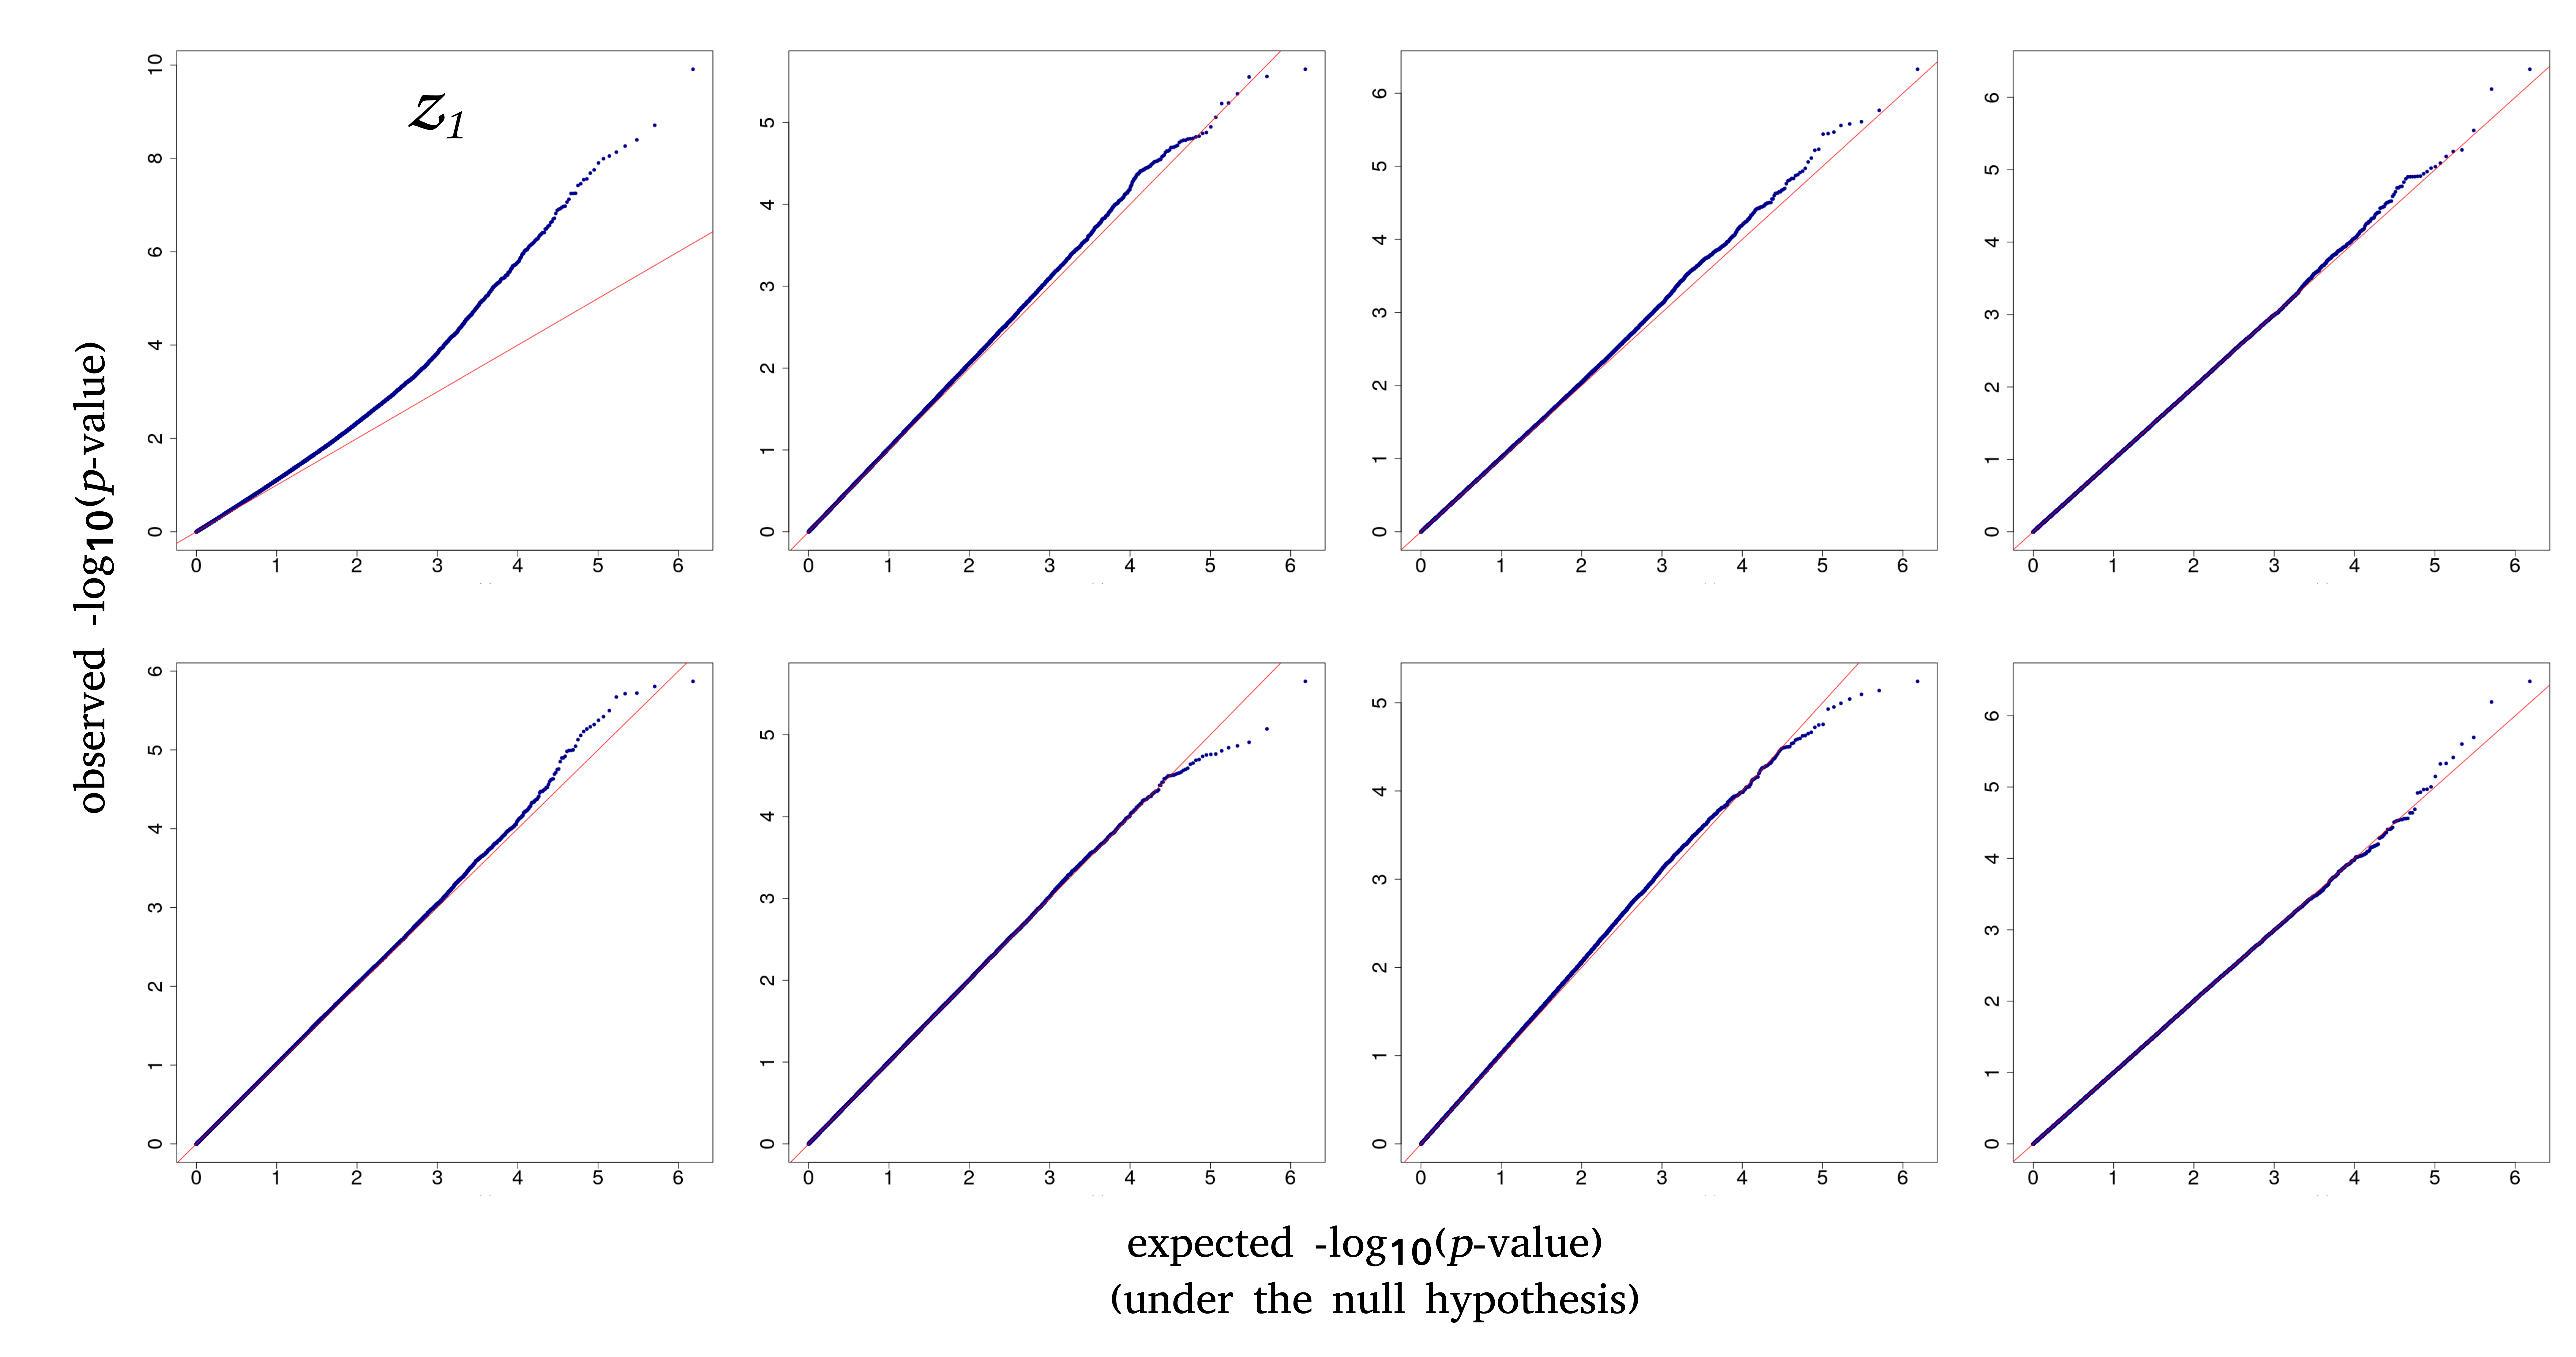
\includegraphics[width=\textwidth]{figs/supplementary/unscaled_qq.png}
 \caption{Q-Q plots for the GWAS on each of the 8 latent variables of unscaled LV meshes (i.e. meshes preserving the original scale from the images). Latent variable $z_1$, presented in the main text, is the only one showing significant associations.}
 \label{fig:qq_unscaled}
\end{figure}

\end{document}


